\documentclass[conference]{IEEEtran}
\IEEEoverridecommandlockouts

\usepackage{cite}
\usepackage{amsmath,amssymb,amsfonts}
\usepackage{booktabs}
\usepackage{graphicx}
\usepackage{textcomp}
\usepackage{xcolor}
\usepackage{hyperref}

\begin{document}

\title{Two-Tier Stance-Guided Signed Graph Neural Networks for Early Cascade Forecasting and Macro Social Network Polarization\thanks{Extended Technical Report formatted in two-column IEEEtran style; secondary benchmarks, diagnostic visualizations, and sensitivity probes are organized in Appendix~\ref{app:extended}.}}

\author{
\IEEEauthorblockN{Vu Hieu Kien}
\IEEEauthorblockA{\textit{Faculty of Information Technology} \\
\textit{Thai Nguyen University of Information and Communication Technology (ICTU)}\\
Thai Nguyen, Vietnam}
\and
\IEEEauthorblockN{Vu Ngoc Anh Thuyen}
\IEEEauthorblockA{\textit{Faculty of Information Technology} \\
\textit{Thai Nguyen University of Information and Communication Technology (ICTU)}\\
Thai Nguyen, Vietnam}
}

\maketitle

\begin{abstract}
Predicting the eventual reach and community polarization of social media discussions alongside macro-scale ideological divisions is challenging due to extreme early-stage structural sparsity, heterophilic conflict edges, target-agnostic profanity, and temporal leakage pitfalls. We present a two-tier signed graph framework combining (i) \textbf{SBi-FAGAT} (\emph{Stance-Guided Bidirectional Frequency-Adaptive Graph Attention Network}), which forecasts final cascade size $y_{\text{size}} = \ln(1 + N_{\text{total}})$ and future stance polarization $y_{\text{polar}} \in [0, 1]$ from the source post and at most $K$ earliest replies ($K=20, N_{\text{reply}} \ge 25$ on Vietnamese Reddit; reduced-horizon $K=10, N_{\text{reply}} \ge 15$ on English PHEME), and (ii) macro cross-thread signed user-interaction networks linking $13{,}718$ users ($85{,}398$ interactions) on Vietnamese Reddit and $50{,}062$ users ($72{,}858$ interactions; $36{,}606$ users in valid reply pairs) on PHEME. Our Natural Language Processing (NLP) pipeline extracts causal \emph{Ancestor-Conditioned SpanPool} node embeddings and distills 2D discourse vectors $e_{uv} = [s_{uv}, h_{uv}]^\top$ via multilingual Natural Language Inference (NLI) verbalizers and class-weighted hostility teachers. Controlled five-seed experiments yield an honest diagnostic contrast across scales. On shallow single-thread Vietnamese Reddit cascades ($N = 225$ Test threads), \texttt{SBiFAGAT} ($R^2_{\text{polar}} = 0.0742$) strongly outperforms an unlearned Early-$K$ Persistence Baseline ($-3.1986$) and matches or trails matched baselines (\texttt{TextMLP} $R^2_{\text{polar}} = 0.0741$; \texttt{TemporalStanceMLP} $0.0608$, Holm--Bonferroni bootstrap $p_{\text{adj}} \ge 0.574$; \texttt{BiEdgeGATv2} $0.0789$ vs.\ ablation Full $0.0777$, $p_{\text{adj}} = 1.00$; \texttt{StandardGCN} MSLE $= 0.1542$ vs.\ $0.1580$; temporal \texttt{FAGCN} $R^2_{\text{size}} = 0.2586$ vs.\ $0.1914$), while on text-free UPFD \texttt{StandardGATv2} outperforms latent-edge \texttt{SBiFAGAT} on GossipCop ($0.9684$ vs.\ $0.9486$, $p_{\text{adj}} = 8.00\text{e-}04$) and \texttt{EdgeGATv2} leads on PolitiFact ($0.8253$ vs.\ $0.8090$, bootstrap $p_{\text{adj}} = 3.20\text{e-}02$). On reduced-horizon PHEME ($N = 334$ Test threads; $5$-fold LOO), \texttt{SBiFAGAT} achieves the top inductive rumor \texttt{Macro-F1} ($0.3541$, bootstrap $p_{\text{adj}} = 8.96\text{e-}02$, paired-$t$ $p_{\text{adj}} = 1.00$) and \texttt{Acc} $= 0.6359$ (bootstrap $p_{\text{adj}} = 7.20\text{e-}03$ vs.\ \texttt{EdgeGATv2} $0.5988$; $+17.2$~pp above the Test-334 \texttt{non-rumor} majority $46.4\%$, while trailing \texttt{TemporalStanceMLP} at $0.6443$), trails \texttt{TextMLP} on $R^2_{\text{polar}}$ ($0.0932$ vs.\ $0.0793$), wins $0/9$ PHEME ablation metrics (trailing \texttt{BiEdgeGATv2} on $R^2_{\text{polar}}$, $0.0791$ vs.\ $0.0940$, bootstrap $p_{\text{adj}} = 8.00\text{e-}03$), and under $5$-fold LOO shift leads on RMSE ($0.0445$), $R^2_{\text{polar}}$ ($0.0512$), \texttt{Macro-F1} ($0.2978$), and \texttt{Acc} ($0.6203$, Exact Perm.\ $p = 0.0625$, $p_{\text{adj}} = 0.5625$) while trailing \texttt{Early-K Persistence} ($0.3171/0.3822$) and \texttt{EdgeGATv2} ($0.2783/0.2783$) on $r/\rho$. Single-author verification of AI-pre-annotated VN pairs ($120$ Test pairs, $30$ trees) and RumourEval-2019 SDQC ($1{,}675$ pairs) further reveals weak silver-label alignment (VN weighted stance accuracy $24.79\%$, $30$-tree $\rho = 0.0018$; RumourEval $2.0\%$--$3.8\%$ minority recall) and \emph{Target-Misattributed Profanity} ($4/7 = 57.1\%$ third-party-cursing supporting replies flipped to opposition). Conversely, lifting the same 2D attributes onto macro user networks exposes sharp spectral separation (VN $Q_{\text{signed}} = 0.4280$, $+19.1$~pp cross-camp opposition, anti-balanced $z = -15.17$; PHEME $Q_{\text{signed}} = 0.8232$ on a sparse $212$-triangle WCC, $+54.5$~pp, RWC $= 0.6218$, $z = -4.30$), where \texttt{SBiFAGAT-Link} shows directional transductive gains on PHEME (\texttt{ROC-AUC} $= 0.9181$, \texttt{PR-AUC} $= 0.7616$, \texttt{Macro-F1} $= 0.8006$; unadjusted paired-$t$ $p = 0.0270$, Exact Perm.\ $p = 0.0625$, $p_{\text{adj}} = 0.1622/0.3750$; $21.7\%$ recurring pairs).
\end{abstract}

\begin{IEEEkeywords}
Graph Neural Networks, Signed Networks, Social Media Polarization, Information Cascades, Stance Detection, Structural Balance
\end{IEEEkeywords}

\section{Introduction}
Online discussions rapidly generate both viral reach and sharp attitudinal division. Forecasting ultimate cascade size $y_{\text{size}} = \ln(1 + N_{\text{total}})$ and future polarization $y_{\text{polar}} \in [0, 1]$ from the earliest interactions while mapping macro community segregation informs early moderation and misinformation triage \cite{zubiaga2016analysing,li2017deepcas,garimella2018quantifying}. Yet learning jointly from Graph Neural Networks (GNNs) and NLP across early cascades confronts three obstacles: (i) standard GNN aggregators assume homophily via low-pass smoothing, washing out heterophilic disagreement signals \cite{bo2021beyond,platonov2023critical}; (ii) unidirectional top-down convolutions ignore how reply subtrees synthesize conflict back toward the root \cite{bian2020rumor}; and (iii) unguarded benchmarks leak post-observation reply counts, future tree depths, or shared topics across splits.

To investigate where signed message passing succeeds and where shallow tree size imposes structural limits, we present an Extended Technical Report detailing a two-tier bilingual framework for Vietnamese Reddit and English PHEME data within $16$~GB GPU and dual Tesla T4 budgets (primary findings appear in Sections~\ref{sec:method}--\ref{sec:results}, with secondary benchmarks, diagnostic visualizations, and edge-sensitivity tables provided in Appendix~\ref{app:extended}):
\begin{enumerate}
    \item \textbf{Strict Early-Cascade Zero-Leakage Contract:} Using Arrow/PyTorch Geometric (PyG) schema validators, all Tier~1 cascade inputs are truncated strictly at $t \le t_K$ ($K=20, N_{\text{reply}} \ge 25$ on Vietnamese Reddit and reduced-horizon $K=10, N_{\text{reply}} \ge 15$ on English PHEME), sharing canonical topic-disjoint splits, Leave-One-Event-Out (LOO) teacher edge isolation, and secret-salted SHA-256 pseudonymization with automated PII scrubbing.
    \item \textbf{Causal SpanPool \& Reply-Span 2D Distillation:} Frozen encoders (\texttt{uitnlp/visobert} \cite{nguyen2023visobert} for Vietnamese; \texttt{cardiffnlp/twitter-roberta-base} \cite{barbieri2020tweeteval} for English) compute ancestor-conditioned reply representations. A multilingual \texttt{mDeBERTa-v3-xnli} stance verbalizer \cite{laurer2024less,he2023debertav3} and class-weighted hostility teachers (\texttt{UIT-ViHSD} \cite{luu2021vihsd} and \texttt{TweetEval-Offensive} \cite{barbieri2020tweeteval}) distill $e_{uv} = [s_{uv}, h_{uv}]^\top$ into a train-split \texttt{DualHeadCrossEncoder}.
    \item \textbf{Dual-Channel Bidirectional SBi-FAGAT:} Paired Top-Down (TD) and Bottom-Up (BU) \texttt{StanceGuidedFAConv} layers combine signed frequency gates $\gamma_{uv}$, unsigned excitation gates $\alpha_{uv}^{\text{exc}}$, Dir-GNN cross-mixing \cite{rossi2023edge}, root-aligned camp dipoles, and a Persistence-Residual logit anchor trained under KL-calibrated optimization.
    \item \textbf{Tier 2 Macro Signed Network \& Multi-Faceted Verification:} Beyond fair five-seed micro comparisons against seven neural baselines, a matched \texttt{BiEdgeGATv2} comparator, Early-$K$ Persistence, external UPFD \cite{dou2021upfd} transfer, RumourEval-2019 SDQC \cite{gorrell2019semeval}, construct correlations (Sarle's Bimodality Coefficient \cite{pfister2013good} and signed assortativity), and observational edge sensitivity probes, we project all valid cross-thread interactions onto a global signed user social network analyzed via Structural Balance Theory \cite{cartwright1956structural}, Signed Laplacian bipartition \cite{kunegis2010spectral}, $Q_{\text{signed}}$, and Random Walk Controversy (RWC) \cite{garimella2018quantifying}, alongside chronological signed link prediction with pre-cutoff feature aggregation.
\end{enumerate}

\section{Related Work}
\subsection{GNNs for Information Cascades, Heterophily, and Signed Graphs}
Homophilic graph networks such as GCN \cite{kipf2017semisupervised} and GATv2 \cite{brody2022how} perform low-pass smoothing, which degrades when neighboring commenters express opposing stances \cite{platonov2023critical}. For cascade size prediction, DeepCas \cite{li2017deepcas} models sampled random-walk diffusion paths rather than explicit edge stance conflict, whereas Bi-GCN \cite{bian2020rumor} models bidirectional tree propagation with root enhancement for rumor classification. Dir-GNN \cite{rossi2023edge} proves that decoupling incoming and outgoing directed transformations strengthens learning on heterophilic topologies. Signed Graph Convolutional Networks (SGCN) \cite{derr2018signed} apply Cartwright--Harary balance paths \cite{cartwright1956structural} to discrete positive/negative links, and FAGCN \cite{bo2021beyond} learns self-gating signed attention coefficients to mix low- and high-frequency signals. SBi-FAGAT extends this lineage to continuous 2D NLP discourse edges $e_{uv} = [s_{uv}, h_{uv}]^\top$ with separate polarity/excitation channels and camp-dipole readouts, while Kunegis et al.~\cite{kunegis2010spectral} provide the Signed Laplacian spectral foundation for our macro network tier.

\subsection{Multilingual Stance Detection and Social Polarization}
Social rumor corpora including PHEME \cite{zubiaga2016analysing,kochkina2018pheme} and SemEval-2019 RumourEval \cite{gorrell2019semeval} evaluate stance across conversation threads using Support, Deny, Query, and Comment (SDQC) categories. Advances in RoBERTa \cite{liu2019roberta}, TweetEval \cite{barbieri2020tweeteval}, DeBERTaV3 \cite{he2023debertav3}, PhoBERT \cite{nguyen2020phobert}, and ViSoBERT \cite{nguyen2023visobert} alongside Vietnamese hate speech resources (UIT-ViHSD \cite{luu2021vihsd}) and multilingual NLI transfer \cite{laurer2024less} enable scalable cross-lingual stance and incivility extraction. At macro user-graph scales, Garimella et al.~\cite{garimella2016quantifying,garimella2018quantifying} quantify echo-chamber segregation via RWC, whereas shallow early trees ($|\mathcal{V}_K| \le 21$ on VN; $|\mathcal{V}_K| \le 11$ on PHEME) are too small for random-walk segregation, motivating our joint micro--macro evaluation paired with Sarle's Bimodality Coefficient \cite{pfister2013good}.

\section{Methodology}\label{sec:method}
\subsection{Data Provenance, Early Formulation, and Zero-Leakage Protocol}
We evaluate two bilingual corpora with strict Tier~1 causal guards:
\begin{itemize}
    \item \textbf{Vietnamese Reddit Corpus:} Public discussions crawled via Arctic Shift from \texttt{r/vozforums} ($87{,}788$ nodes) and \texttt{r/VietNam} ($32$ nodes; $99.96\%$ \texttt{r/vozforums}), with source posts spanning 2025-06-15 to 2025-11-14 UTC and reply activity extending through 2026-06-04 UTC ($87{,}820$ total nodes, $86{,}320$ edges across $1{,}500$ cascades with $N_{\text{reply}} \ge 25$, median $44.0$ and mean $57.5$ replies, median duration $95.22$~h). Because Reddit lacks shared external event labels, Train/Val/Test ($1{,}050/225/225$) uses a heuristic 30-day temporal-window and TF-IDF cosine ($\ge 0.30$) topic grouping yielding $1{,}496$ clusters, audited against a strict chronological temporal holdout ($225$ Test cascades).
    \item \textbf{English PHEME Corpus (Reduced Horizon):} $6{,}425$ raw Twitter rumor threads ($101{,}342$ nodes, $94{,}917$ edges across $9$ news events; $1{,}067$ true, $697$ unverified, $638$ false, $4{,}023$ non-rumor; raw median $11.0$ replies, median span $2.53$~h), yielding $2{,}664$ eligible cascades ($414$ true, $270$ unverified, $162$ false, $1{,}818$ non-rumor, i.e., $68.2\%$ non-rumor across the full eligible cohort; median $20.0$ and mean $27.9$ replies, median duration $5.09$~h) under the reduced observation horizon $K=10, N_{\text{reply}} \ge 15$. Cascades are partitioned canonically by event into Train/Val/Test ($1{,}786/544/334$ across all $9$ events; Test-334 holds $155$ non-rumor [$46.4\%$], $131$ true, $27$ false, and $21$ unverified across \texttt{ottawashooting} and \texttt{prince-toronto}) with linear-amplitude future polarization targets (corpus mean $y_{\text{polar}} = 0.0719 \pm 0.0464$), alongside $5$-fold LOO evaluation across the five events with $\ge 15$ eligible cascades (\texttt{charliehebdo}, \texttt{ferguson}, \texttt{germanwings-crash}, \texttt{ottawashooting}, \texttt{sydneysiege}).
\end{itemize}

For each early graph $\mathcal{G}_K = (\mathcal{V}_K, \mathcal{E}_K^{\text{TD}}, \mathcal{E}_K^{\text{BU}})$ retaining only the root and earliest $K$ chronological replies ($t \le t_K$, with $K=20$ for VN and $K=10$ for PHEME), every node $v \in \mathcal{V}_K$ carries $x_v = [\mathbf{e}_v^{\text{Span}} \Vert t_{\text{norm}}(v) \Vert d_{\text{norm}}(v)] \in \mathbb{R}^{770}$, where $t_{\text{norm}}(v) = \min\!\bigl(1, \ln(1 + \Delta t_v)/\ln(1 + T_{\text{ref}})\bigr)$ with elapsed seconds $\Delta t_v$ since the root post, fixed horizon $T_{\text{ref}} = 604{,}800$~s (7 days), and $d_{\text{norm}}(v) = \min\!\bigl(1, \operatorname{depth}(v)/K\bigr)$, paired with a $10$-D causal structural tensor $\mathbf{s}_v^{\text{struct}} \in [0, 1]^{10}$ and an $8$-D cascade summary vector $c_{\mathcal{G}} \in [0, 1]^8$ (Table~\ref{tab:features}). All inputs strictly exclude post-$t_K$ timestamps, full-tree degrees, or global label statistics. Unobserved post-horizon replies ($t > t_K$, count $n \ge 2$) and total full-tree reply count $N_{\text{total}}$ define continuous regression targets:
\begin{multline}
y_{\text{size}} = \ln(1 + N_{\text{total}}), \\
y_{\text{polar}} = \operatorname{clip}\!\Biggl(\lambda_p \min\!\bigl(1, s_{\tilde{s}}\bigr) \\
+ (1-\lambda_p)\min\!\left(1, 2\sqrt{\frac{n}{n-1} m_+ m_-}\right),\, 0,\, 1\Biggr),
\end{multline}
where $\lambda_p = 0.5$, $\tilde{s}_{\text{root}} = +1$, and $\tilde{s}_v \in [-1, 1]$ is the root-aligned future stance---assigned directly from $(\text{root}, v)$ NLI predictions when available for depth $\ge 2$ replies to avoid multi-hop sign drift, and otherwise propagated via breadth-first traversal $\tilde{s}_v = \operatorname{clip}(\tilde{s}_{\operatorname{par}(v)}/\epsilon_0, -1, 1) \cdot s_{\operatorname{par}(v),v}$ with neutral attenuation band $\epsilon_0 = 0.1$---while $m_+ = \frac{1}{n}\sum_v \max(\tilde{s}_v, 0)$, $m_- = \frac{1}{n}\sum_v \max(-\tilde{s}_v, 0)$, and $s_{\tilde{s}} = \sqrt{\frac{1}{n-1}\sum_v (\tilde{s}_v - \bar{\tilde{s}})^2}$ is the unbiased sample standard deviation of $\tilde{s}_v$; the Bessel factor $\frac{n}{n-1}$ removes finite-sample covariance bias prior to square-root linear amplitude scaling. On PHEME, models also predict 4-class veracity $y_{\text{rumor}}$. As a non-learned comparator, \textbf{Early-$K$ Persistence} predicts $y_{\text{size}}$ as the Train-split mean log-size and $y_{\text{polar}}$ by evaluating Eq.~(1) directly on the observed early tree $\mathcal{G}_K$ (BFS orientations without direct root override).

\begin{table}[t]
\centering
\caption{Causal Early-Window Structural Descriptors ($\mathbf{s}_v^{\text{struct}} \in [0,1]^{10}$) and Cascade Burst-Velocity Summary ($c_{\mathcal{G}} \in [0,1]^8$) Extracted Strictly on $\mathcal{G}_K$.}
\label{tab:features}
\resizebox{\columnwidth}{!}{
\begin{tabular}{lp{5.8cm}}
\toprule
Vector & Feature Components ($t \le t_K$, Bounded in $[0, 1]$) \\
\midrule
$\mathbf{s}_v^{\text{struct}}$ (10-D) & (0) $t_{\text{norm}}$ root lag; (1) normalized parent--reply log lag $\Delta t_{\text{par}}$; (2) relative horizon arrival phase $\Delta t_v / t_K$; (3) chronological rank $i/K$; (4) $d_{\text{norm}}$; (5) \texttt{is\_root}; (6) normalized early out-degree in $\mathcal{V}_K$; (7) \texttt{is\_early\_leaf}; (8) root-author re-entry indicator; (9) cumulative author repeat count $/K$. \\
\midrule
$c_{\mathcal{G}}$ (8-D) & (0) normalized horizon elapsed span; (1) mean normalized inter-arrival gap; (2) logistic burst acceleration $\sigma\bigl(\ln(1+\bar{g}_{\text{early}}) - \ln(1+\bar{g}_{\text{late}})\bigr)$ using early/late half mean inter-reply gaps $\bar{g}_{\text{early}},\bar{g}_{\text{late}}$ ($\sigma$: logistic sigmoid); (3) direct-to-root reply fraction; (4) max early tree depth $/K$; (5) unique hashed author ratio; (6) substantive reply fraction ($\ge 8$ tokens); (7) one-sided hostility index ($|\bar{s}_{uv}|\cdot\bar{h}_{uv}$). \\
\bottomrule
\end{tabular}
}
\end{table}

\subsection{Offline Ancestor-Conditioned SpanPool and 2D Distillation}
To decouple transformer memory from five-seed GNN training, frozen backbones (\texttt{uitnlp/visobert} for VI, \texttt{cardiffnlp/twitter-roberta-base} for EN) encode causal paths up to $256$ tokens (\texttt{[CLS] root [SEP] reply [SEP]} at depth $1$, omitting duplicate parent tokens, and \texttt{[CLS] root [SEP] parent [SEP] reply [SEP]} at depth $\ge 2$, with 60/40 head--tail truncation on long roots) and mean-pool exclusively over reply tokens to obtain $\mathbf{e}_v^{\text{Span}} \in \mathbb{R}^{768}$ (whereas pairwise NLI teachers use $384$-token windows). Pairwise 2D discourse attributes $e_{uv} = [s_{uv}, h_{uv}]^\top \in [-1, 1] \times [0, 1]$ are scored by two teachers:
\begin{itemize}
    \item \textbf{Symmetric NLI Stance Teacher ($s_{uv}$):} Evaluating paired NLI hypotheses (entailment, neutral, and contradiction triples $(e_{\text{sup}}, n_{\text{sup}}, c_{\text{sup}})$ and $(e_{\text{opp}}, n_{\text{opp}}, c_{\text{opp}})$ for supporting vs.\ opposing the target claim under a 384-token reply-preserving budget), double contradictions $m_{\text{dc}} = \min(c_{\text{sup}}, c_{\text{opp}})$ are subtracted prior to symmetric averaging: $p_{\text{sup}} = \tfrac{1}{2}(e_{\text{sup}} + (c_{\text{opp}} - m_{\text{dc}})_+)$, $p_{\text{opp}} = \tfrac{1}{2}(e_{\text{opp}} + (c_{\text{sup}} - m_{\text{dc}})_+)$, and $p_{\text{neu}} = \tfrac{1}{2}(n_{\text{sup}} + n_{\text{opp}}) + m_{\text{dc}}$, defining $s_{uv} = p_{\text{sup}} - p_{\text{opp}} \in [-1, 1]$.
    \item \textbf{Class-Weighted Hostility Teacher ($h_{uv}$):} Inverse-frequency square-root class weighting fine-tunes \texttt{uitnlp/visobert} on UIT-ViHSD \cite{luu2021vihsd} (VI), alongside \texttt{twitter-roberta-base-offensive} \cite{barbieri2020tweeteval} (EN).
    \item \textbf{Cross-Encoder Distillation:} Strictly within $\mathcal{T}_{\text{train}}$, a shared-encoder \texttt{DualHeadCrossEncoder} processes the interaction vector $[\mathbf{h}_{\text{CLS}} \Vert \mathbf{h}_{\text{ctx}} \Vert \mathbf{h}_{\text{reply}} \Vert \mathbf{h}_{\text{ctx}} \odot \mathbf{h}_{\text{reply}} \Vert |\mathbf{h}_{\text{ctx}} - \mathbf{h}_{\text{reply}}|]$ (from the \texttt{[CLS]} representation and mean-pooled context/reply span embeddings in $\mathbb{R}^{768}$) for stance and reply-span pooling for $h_{uv}$ (preventing parent profanity bleed), optimized with temperature-scaled 3-class Kullback--Leibler divergence $T^2 \cdot \operatorname{KL}_T$ ($T=2.0$) over $(p_{\text{sup}}, p_{\text{neu}}, p_{\text{opp}})$, $0.5\,\operatorname{SmoothL1}$ ($\beta=0.1$) on $s_{uv}$, and binary cross-entropy (\texttt{BCEWithLogits}) on $h_{uv}$. Canonical inductive evaluation uses student scores; LOO and temporal holdout protocols isolate evaluation using teacher edges.
\end{itemize}

\subsection{Tier 1 SBi-FAGAT Architecture and Optimization}
A shared \texttt{TwoStreamNodeStem} encodes the semantic embedding $\mathbf{e}_v^{\text{Span}} \in \mathbb{R}^{768} \to \mathbb{R}^{48}$ and structural tensor $\mathbf{s}_v^{\text{struct}} \in \mathbb{R}^{10} \to \mathbb{R}^{16}$ through separate \texttt{Linear+GELU+LayerNorm} projections concatenated into $\mathbf{h}_v^{(0)} \in \mathbb{R}^{d}$ ($d=64$ across all models; $L=2$ message-passing layers for all GNNs; initialized identically as $\mathbf{h}_v^{\xi,(0)} = \mathbf{h}_v^{(0)}$ for both streams $\xi \in \{\text{TD}, \text{BU}\}$). For graph-agnostic \texttt{TextMLP}, topology columns $\{1, 4, 6, 7\}$ in $\mathbf{s}_v^{\text{struct}}$ and topology/hostility columns $\{3, 4, 7\}$ in $c_{\mathcal{G}}$ are zero-masked; \texttt{TemporalStanceMLP} retains node temporal-structural features and fuses root and mean-pooled node embeddings with pooled per-graph 2D edge statistics (mean, standard deviation, minimum, and maximum of $e_{uv}$; $8$ scalars) through an MLP before the shared head. Among edge-aware GNN comparators, \texttt{EdgeGATv2} augments \texttt{GATv2Conv} with edge vector $e_{uv}$ on undirected edges; \texttt{BiEdgeGATv2} matches \texttt{SBi-FAGAT}'s coupled TD+BU streams, 2D edge inputs, and global attention readout using standard \texttt{GATv2Conv} layers in place of dual-channel signed gates and the Camp Dipole module; and on UPFD (which lacks reply text for pairwise NLI), \texttt{LatentConflictMLP} synthesizes $2$-D edge proxies $\mathbf{e}_{\text{latent}} = \operatorname{MLP}([\mathbf{x}_u \Vert \mathbf{x}_v \Vert \mathbf{x}_u - \mathbf{x}_v])$ from adjacent node pairs.

Inside each \texttt{StanceGuidedFAConv} layer ($l \in \{1, \dots, L\}$) over directional stream $\xi \in \{\text{TD}, \text{BU}\}$ (opposite stream $\bar{\xi}$; reversed BU edges $(v \to u)$ reuse parent-to-reply attributes $e_{uv}$), linear projections $\mathbf{z}_u^{\xi,(l)} = \mathbf{W}^{\xi,(l)} \mathbf{h}_u^{\xi,(l-1)}$ and LayerNorm (\texttt{LN}) normalized vectors $\mathbf{z}_u^{\xi,\text{norm},(l)} = \operatorname{LN}(\mathbf{z}_u^{\xi,(l)})$ drive a signed polarity gate $\gamma_{uv}^{\xi,(l)} \in (-1, 1)$ (Xavier node gain $0.2$, initial cosine weight $\omega^{\xi,(l),(0)} = 0.10$) and an unsigned excitation gate $\alpha_{uv}^{\text{exc},(l)} \in (0, 1)$, splitting $\mathbf{z}_u^{\xi,(l)} = [(\mathbf{z}_u^{\xi,\text{pol},(l)})^\top, (\mathbf{z}_u^{\xi,\text{exc},(l)})^\top]^\top$ evenly into two $\mathbb{R}^{d/2}$ channels:
\begin{multline}
\gamma_{uv}^{\xi,(l)} = \tanh\!\Biggl(\frac{(\mathbf{a}_{\text{node}}^{\xi,(l)})^\top [\mathbf{z}_u^{\xi,\text{norm},(l)} \Vert \mathbf{z}_v^{\xi,\text{norm},(l)}]}{\sqrt{2d}} \\
+ \omega^{\xi,(l)} \cos(\mathbf{z}_u^{\xi,\text{norm},(l)}, \mathbf{z}_v^{\xi,\text{norm},(l)}) \\
+ (\mathbf{a}_{\text{edge}}^{\xi,(l)})^\top e_{uv} + \delta_{\gamma}^{\xi,(l)}(e_{uv})\Biggr),
\end{multline}
\begin{multline}
\alpha_{uv}^{\text{exc},(l)} = \sigma\bigl(0.8|s_{uv}| + 0.8 h_{uv} + \delta_{\alpha}^{\xi,(l)}(e_{uv})\bigr), \\
\phi_{uv}^{\xi,(l)}(\mathbf{z}_u^{\xi,(l)}) = \begin{bmatrix} \gamma_{uv}^{\xi,(l)}\, \mathbf{z}_u^{\xi,\text{pol},(l)} \\ \alpha_{uv}^{\text{exc},(l)}\, \mathbf{z}_u^{\xi,\text{exc},(l)} \end{bmatrix},
\end{multline}
where $\sigma(\cdot)$ is the logistic sigmoid and $\delta_{\gamma}^{\xi,(l)}, \delta_{\alpha}^{\xi,(l)}$ are outputs of a two-layer Gaussian Error Linear Unit (GELU) edge basis network over $[s_{uv}, h_{uv}, s_{uv} h_{uv}, |s_{uv}|]^\top$. Under symmetric degree normalization $c_{uv}^{\xi} = \sqrt{(d_{\text{out}}^{\xi}(u)+1)(d_{\text{in}}^{\xi}(v)+1)}$ in $(\mathcal{V}_K, \mathcal{E}_K^\xi)$, layer updates combine aggregated messages $\mathbf{m}_v^{\xi,(l)} = \sum_{u \in \mathcal{N}^{\xi}(v)} \frac{1}{c_{uv}^{\xi}}\phi_{uv}^{\xi,(l)}(\mathbf{z}_u^{\xi,(l)})$, initial residual $\epsilon = 0.5$ (distinct from BFS neutral band $\epsilon_0 = 0.1$), root broadcast, odd-symmetric stabilization with dropout, and Dir-GNN directional cross-mixing ($\eta_l^{(0)} = 0.10$) \cite{rossi2023edge}:
\begin{multline}
\mathbf{r}_v^{\xi,(l)} = 0.5 \mathbf{h}_v^{\xi,(l-1)} + \epsilon \mathbf{h}_v^{(0)} + \mathbf{m}_v^{\xi,(l)} + \mathbf{W}_{\text{root}}^{\xi,(l)} \mathbf{h}_{\text{root}}^{(0)} + \mathbf{b}_{\text{root}}^{\xi,(l)}, \\
\tilde{\mathbf{h}}_v^{\xi,(l)} = \operatorname{Dropout}\!\Bigl(\operatorname{LN}\!\bigl(\mathbf{r}_v^{\xi,(l)} + 0.2\tanh(\mathbf{r}_v^{\xi,(l)})\bigr)\Bigr), \\
\mathbf{h}_v^{\xi,(l)} = \tilde{\mathbf{h}}_v^{\xi,(l)} + \tanh(\eta_l) \mathbf{W}_{\text{mix}}^{\xi,(l)} \tilde{\mathbf{h}}_v^{\bar{\xi},(l)}.
\end{multline}

After $L=2$ layers, directional node states merge symmetrically as $\mathbf{h}_v = \tfrac{1}{2}(\mathbf{h}_v^{\text{TD},(L)} + \mathbf{h}_v^{\text{BU},(L)})$, root embedding $\mathbf{z}_{\text{root}} = \tfrac{1}{2}(\mathbf{h}_{\text{root}}^{\text{TD},(L)} + \mathbf{h}_{\text{root}}^{\text{BU},(L)})$, and global softmax attention pooling averages per-stream readouts $\mathbf{z}_{\text{att}} = \tfrac{1}{2}\bigl(\operatorname{Attn}_{\text{TD}}(\{\mathbf{h}_v^{\text{TD},(L)}\}) + \operatorname{Attn}_{\text{BU}}(\{\mathbf{h}_v^{\text{BU},(L)}\})\bigr)$, forming $\mathbf{z}_{\text{base}} = [\mathbf{z}_{\text{root}} \Vert \mathbf{z}_{\text{att}}] \in \mathbb{R}^{2d}$. A Camp Dipole bottleneck ($\operatorname{MLP}_{\text{dip}}\!: \mathbb{R}^{3d+6} \to \mathbb{R}^{d/2} \to \mathbb{R}^{2d}$) modulates $\mathbf{z}_{\text{base}}$ via $\beta_{\text{dip}}^{(0)} = 0.25$:
\begin{multline*}
\mathbf{z}_{\text{graph}} = \operatorname{LN}\!\Bigl(\mathbf{z}_{\text{base}} + \tanh(\beta_{\text{dip}})\operatorname{MLP}_{\text{dip}}\!\bigl([\mathbf{z}_{\text{disp}} \\
\Vert \mathbf{z}_{\text{dipole}}^{\text{polar}} \Vert \mathbf{z}_{\text{dipole}}^{\text{signed}} \Vert \mathbf{g}_{\text{mom}}]\bigr)\Bigr),
\end{multline*}
where $\mathbf{z}_{\text{disp}} = \sqrt{\operatorname{Var}_v(\mathbf{h}_v) + 10^{-6}} \in \mathbb{R}^{d}$ is per-cascade feature standard deviation. Running $64$-hop root-aligned BFS ($\epsilon_0 = 0.1$) over last-layer TD gates $\gamma_{uv}^{\text{TD},(L)}$ yields aligned edge orientations $\hat{\gamma}_{uv} \in [-1, 1]$, destination camp weights $w_\pm(v) = \operatorname{ReLU}(\pm\hat{\gamma}_{uv})$ ($u = \operatorname{par}(v)$), normalized camp fractions $f_\pm = (\sum_{v} w_\pm(v))/|\mathcal{E}_K^{\text{TD}}|$, and weighted camp centroids $\boldsymbol{\mu}_\pm = \sum_v w_\pm(v)\mathbf{h}_v / \sum_v w_\pm(v)$. These form $\mathbf{z}_{\text{dipole}}^{\text{polar}} = b\sqrt{(\boldsymbol{\mu}_+ - \boldsymbol{\mu}_-)^2 \mathbb{I}[\text{both}] + 10^{-8}} \in \mathbb{R}^{d}$ and $\mathbf{z}_{\text{dipole}}^{\text{signed}} = (\boldsymbol{\mu}_+ - \boldsymbol{\mu}_-)\mathbb{I}[\text{both}] \in \mathbb{R}^{d}$ ($b = 2\mathbb{I}[\text{both}]\sqrt{\operatorname{clip}(f_+ f_-, 0, 0.25) + 10^{-8}}$, zeroed when either camp lacks mass), while $\mathbf{g}_{\text{mom}} \in \mathbb{R}^6$ stacks three raw $\gamma_{uv}^{\text{TD},(L)}$ statistics (mean, standard deviation, mean absolute value) with BFS-aligned camp moments $(f_+, f_-, b)$. Within \texttt{MultiTaskHead}, $c_{\mathcal{G}}$ passes through a cascade projection ($\mathbb{R}^8 \to \mathbb{R}^{32}$) concatenated with $\mathbf{z}_{\text{graph}}$ only for size and veracity heads, whereas the polarization head decodes $\Delta z_{\text{polar}}$ solely from $\mathbf{z}_{\text{graph}}$ (so ablating $c_{\mathcal{G}}$ affects $R^2_{\text{polar}}$ only via shared-trunk gradients), adding a zero-initialized Persistence-Residual anchor for stance-aware models:
\begin{multline}
z_{\text{polar}} = \tanh(w_p)\bigl(\operatorname{logit}(\operatorname{clip}(y_{\text{polar}}^{\text{early}}(\mathcal{G}_K), 0.02, 0.98)) \\
- \bar{\ell}_{\text{train}}\bigr) + \Delta z_{\text{polar}},
\end{multline}
where $\bar{\ell}_{\text{train}} = \operatorname{mean}_{\text{train}}(\operatorname{logit}(\operatorname{clip}(y_{\text{polar}}^{\text{early}}, 0.02, 0.98)))$ centers the anchor logit on the Train split. To avoid sigmoid tail gradient vanishing on continuous $y_{\text{polar}} \in [0, 1]$, we minimize zero-minimum KL-calibrated binary cross-entropy combined with Smooth-L1 ($\beta = 0.05$):
\begin{multline}
\mathcal{L}_{\text{polar}} = \bigl(\operatorname{BCEWithLogits}(z_{\text{polar}}, y_{\text{polar}}) - H(y_{\text{polar}})\bigr)_+ \\
+ \operatorname{SmoothL1}(\sigma(z_{\text{polar}}), y_{\text{polar}}),
\end{multline}
where $H(p) = -p\ln p - (1-p)\ln(1-p)$ is binary Shannon entropy and $(\cdot)_+ = \max(0, \cdot)$, paired with Huber regression on $y_{\text{size}}$ and dampened square-root class-weighted cross-entropy on PHEME $y_{\text{rumor}}$ (heteroscedastic uncertainty weighting disabled, $\lambda_{\text{unc}} = 0$, in fixed benchmarks), Train-only 2:1 normalized task scaling (normalizing $\mathcal{L}_{\text{size}}$ and $\mathcal{L}_{\text{polar}}$ by Train constant-mean baseline losses at $1.0 : 0.5$ weight ratio), and Train mean-target output bias initialization. All Tier~1 neural models share identical optimization: AdamW (learning rate $10^{-3}$, weight decay $10^{-4}$, dropout $0.1$, gradient clipping norm $5.0$), batch size $32$ ($64$ on UPFD), up to $100$ epochs with $5$-epoch linear warmup and \texttt{ReduceLROnPlateau} (factor $0.5$, patience $5$, minimum LR $2\times 10^{-5}$), EMA ($\text{decay}=0.985$), validation early stopping (patience $10$ on task loss), validation-only comparator selection, and deterministic evaluation across seeds $[42, 100, 2024, 777, 999]$.

\subsection{Tier 2 Macro Signed User-Interaction Social Network}
To bridge isolated early trees with global community structure without additional data collection, we project all valid non-deleted, non-self-loop user reply interactions $(u, v)$ across cascades onto a global signed social graph $\mathcal{G}_{\text{macro}} = (\mathcal{U}, \mathcal{E}_{\text{user}})$. Two complementary analyses operate on $\mathcal{G}_{\text{macro}}$:
\begin{itemize}
    \item \textbf{Macro Polarization Geometry:} Undirected user pairs with mean stance $|\bar{s}_{uv}| \ge 0.1$ induce signed weights $w_{uv} = \operatorname{sign}(\bar{s}_{uv}) |\bar{s}_{uv}| \ln(1 + c_{uv})$ over $c_{uv}$ interactions (and symmetric signed matrix $W$ with diagonal unsigned strength $\bar{D}_{uu} = \sum_v |W_{uv}|$). On the largest undirected strong-pair Weakly Connected Component (WCC), we extract the smallest eigenvector of the normalized Signed Laplacian \cite{kunegis2010spectral} $\bar{L}_{\text{signed}} = I - \bar{D}^{-1/2} W \bar{D}^{-1/2}$ (falling back to the second eigenvector's median split only if a camp falls below $5\%$ of WCC size) to bipartition users into two latent camps $(\mathcal{C}_0, \mathcal{C}_1)$, evaluating (a) Structural Balance \cite{cartwright1956structural} balanced triangle fraction $(N_{+++} + N_{+--})/N_{\triangle}$ and its $z$-score against $100$ uniform edge-sign permutations, (b) Signed Modularity $Q_{\text{signed}} = Q^+ - Q^-$, where for sign subgraph $\tau \in \{+, -\}$ with positive total edge weight $m^\tau = \sum_{(u,v)\in \mathcal{E}^\tau} |w_{uv}|$ and unsigned incident degree $k_u^\tau = \sum_{v:(u,v)\in \mathcal{E}^\tau} |w_{uv}|$,
    \[
    Q^\tau = \frac{1}{m^\tau}\sum_{\substack{(u,v)\in \mathcal{E}^\tau \\ c_u = c_v}} |w_{uv}| - \frac{1}{4(m^\tau)^2}\sum_{r \in \{0, 1\}}\left(\sum_{u \in \mathcal{C}_r} k_u^\tau\right)^{\!2},
    \]
    (c) Garimella RWC \cite{garimella2018quantifying} via absorbing random walks between top-degree camp hubs ($\alpha = 0.85$, restarting teleport mass back to the originating camp's seed distribution; evaluated over positive WCC edges and falling back to all WCC interactions whenever $|\mathcal{E}^+_{\text{WCC}}| < |\mathcal{V}_{\text{WCC}}|$ or for WCC nodes with zero positive degree), and (d) within- vs.\ cross-camp opposition and incivility rates.
    \item \textbf{Chronological Signed Link Prediction:} All signed interactions ($|s_{uv}| \ge 0.1$) are partitioned chronologically ($70\%/15\%/15\%$) at non-overlapping UTC cutpoints $t_{\text{train}} < t_{\text{val}} < t_{\text{test}}$. Node features $x_u^{\text{macro}} = [\bar{\mathbf{e}}_u^{\text{Span}} \Vert \mathbf{a}_u^{\text{4D}}] \in \mathbb{R}^{772}$ aggregate pre-cutoff ($t \le t_{\text{train}}$) post embeddings and 4-D unsigned log-activity counts (posts, cascades, out-replies, in-replies; zeroed for cold-start Test users with zero pre-cutoff posts, though unseen Test users absent from signed Train edges still retain non-zero pre-cutoff embeddings/activity when appearing in neutral $|s_{uv}| < 0.1$ or sub-threshold threads). During training mini-batches, unordered target pairs $\{u, v\}$ are masked out of Train message passing; during validation and testing, the full Train graph is passed unmasked (allowing recurring $\{u, v\}$ pairs to read prior Train edges). We benchmark six equal-width ($d=64, L=2$) architectures (\texttt{UserTextMLP}, \texttt{StandardGCN}, \texttt{StandardGATv2}, \texttt{SGCN} \cite{derr2018signed}, \texttt{FAGCN} \cite{bo2021beyond}, and \texttt{SBiFAGAT-Link}) over 5 seeds predicting opposing ($s_{uv} \le -0.1$) vs.\ supporting links. \texttt{SBiFAGAT-Link} maps $x_u^{\text{macro}}$ via a two-stream \texttt{UserNodeStem}, runs $L=2$ bidirectional \texttt{StanceGuidedFAConv} layers over forward $(u, v)$ and reversed $(v, u)$ Train edges fused via GELU residual mixing, and scores pairs with a \texttt{PairwiseSignedHead} MLP over $[\mathbf{h}_u \Vert \mathbf{h}_v \Vert \mathbf{h}_u \odot \mathbf{h}_v \Vert |\mathbf{h}_u - \mathbf{h}_v|]$ (AdamW, LR $10^{-3}$, up to $40$ epochs, batch size $1{,}024$, patience $8$ on Val ROC-AUC, Val-tuned Macro-F1 threshold, positive-weighted BCE). Notably, only \texttt{SBiFAGAT-Link} consumes continuous 2D edge attributes $e_{uv} = [s_{uv}, h_{uv}]^\top$, whereas \texttt{SGCN} consumes discrete signs $\operatorname{sign}(s_{uv})$ and the remaining baselines ignore edge attributes.
\end{itemize}

\section{Experimental Setup}
All neural models share fixed hidden width ($d=64$) and matched $128$-D regression heads evaluated over five deterministic seeds, reporting paired $t$-tests, nonparametric bootstrap $p$-values (exact two-sided sign-flip permutation for $F=5$ LOO event folds and 5-seed Tier~2 link prediction, where the mathematical minimum two-sided $p$-value is $2/2^5 = 0.0625$), and Holm--Bonferroni corrections against the strongest validation-selected comparator. For VN ($225$ Test cascades across $>6$ clusters), bootstrap draws resample topic clusters; for PHEME ($334$ Test cascades across only $2$ held-out events, $<6$ clusters), cluster bootstrap falls back to fixed-seed cascade-level IID bootstrap over averaged 5-seed predictions, so $^{**}$ markers on PHEME tables indicate within-event cascade bootstrap rather than cross-event significance (all paired 5-seed $t$-tests yield Holm--Bonferroni $p_{\text{adj}} = 1.00$). Table~\ref{tab:dataset_eda} summarizes exploratory corpus splits and Early-$K$ Persistence performance directly from validated dataset tables.

\IfFileExists{tables_dataset_eda.tex}{
  \begin{table*}[t]
\centering
\caption{Exploratory dataset statistics (PHEME: $K=10, N_{\text{reply}} \ge 15$, VN: $K=20, N_{\text{reply}} \ge 25$) and Early-$K$ Persistence Baseline on Test splits.}
\label{tab:dataset_eda}
\resizebox{\textwidth}{!}{
\begin{tabular}{lcccccccc}
\toprule
Dataset & Raw & Forecast Eligible & Topics & Train/Val/Test & Med (Mean) Replies & Med Span (h) & Persist RMSE$\downarrow$ & Persist $r$$\uparrow$ \\
\midrule
pheme ($K{=}10, \ge 15$) & 6,425 & 2,664 & 9 & 1786/544/334 & 20.0 (27.9) & 5.09 & 0.0562 & 0.3310 \\
vn ($K{=}20, \ge 25$) & 1,500 & 1,500 & 1,496 & 1050/225/225 & 44.0 (57.5) & 95.22 & 0.0788 & 0.0217 \\
\bottomrule
\end{tabular}
}
\end{table*}

}{
  \IfFileExists{tables_dataset_eda_pheme.tex}{\input{tables_dataset_eda_pheme}}{}
  \IfFileExists{tables_dataset_eda_vn.tex}{\input{tables_dataset_eda_vn}}{}
}

\section{Results and Analysis}\label{sec:results}
\subsection{Vietnamese Early-Cascade Inductive and Temporal Holdout}
On the $225$-cascade Vietnamese Reddit Test split (Table~\ref{tab:main_vn}), non-learned Early-$K$ Persistence collapses to $R^2_{\text{polar}} = -3.1986$ (RMSE $= 0.0788$, $r = 0.0217$), whereas all neural models achieve positive explained variance. \texttt{SBiFAGAT} attains the top $R^2_{\text{polar}} = 0.0742 \pm 0.0157$ (RMSE $= 0.0370 \pm 0.0003$, $r = 0.2899$, $\rho = 0.2272$), essentially matching graph-agnostic \texttt{TextMLP} ($R^2_{\text{polar}} = 0.0741 \pm 0.0181$, $r = 0.2989$, $\rho = 0.2501$) and \texttt{EdgeGATv2} ($0.0689$), with Holm--Bonferroni bootstrap $p_{\text{adj}} \ge 0.574$ vs.\ validation-selected \texttt{TemporalStanceMLP} ($0.0608$). For early size prediction, \texttt{StandardGCN} ($0.1542 \pm 0.0048$, $R^2_{\text{size}} = 0.3097$) leads while \texttt{SBiFAGAT} obtains $0.1580$ ($R^2_{\text{size}} = 0.2926$). Figure~\ref{fig:umap_vn} (Appendix~\ref{app:diagnostics}) contrasts UMAP node projections on the VN test split.

Under strict chronological VN temporal holdout using the teacher-isolated edge protocol ($225$ Test cascades; Table~\ref{tab:temporal_vn} in Appendix~\ref{app:micro_ext}), Early-$K$ Persistence degrades further ($R^2_{\text{polar}} = -5.4386$), whereas all learned architectures maintain $R^2_{\text{polar}} \in [0.0481, 0.0815]$: \texttt{SBiFAGAT} obtains the strongest polarization rank correlation ($\rho = 0.3058 \pm 0.0187$, $r = 0.3338$), trailing \texttt{TemporalStanceMLP} ($R^2_{\text{polar}} = 0.0815$, $p_{\text{adj}} = 1.00$) and \texttt{FAGCN} on size ($0.1881$ vs.\ $0.2051$ MSLE). Practically, on shallow single-thread trees ($|\mathcal{V}_K| \le 21$) with weak topic clustering ($1{,}496/1{,}500$), frozen ancestor-conditioned NLP embeddings already capture nearly all predictive signal available to early GNNs.

\IfFileExists{tables_main_vn.tex}{\begin{table*}[t]
\centering
\caption{Vietnamese Reddit (VN) Early Cascade Size and Future Polarization Forecasting at $K=20, N_{\text{reply}} \ge 25$ (Inductive, Mean $\pm$ Std, using Persistence Anchor and 8-D Burst Stats). Stars indicate significance vs.\ TemporalStanceMLP ($^{*}p<0.05$, $^{**}p<0.01$).}
\label{tab:main_vn}
\resizebox{\textwidth}{!}{
\begin{tabular}{lccccccc}
\toprule
Model & MSLE $\downarrow$ & MAE $\downarrow$ & $R^2_{\text{size}}$ $\uparrow$ & RMSE $\downarrow$ & $R^2_{\text{polar}}$ $\uparrow$ & Pearson $r$ $\uparrow$ & Spearman $\rho$ $\uparrow$ \\
\midrule
Early-K Persistence & 0.2285 $\pm$ 0.0000 & 0.3872 $\pm$ 0.0000 & -0.0232 $\pm$ 0.0000 & 0.0788 $\pm$ 0.0000 & -3.1986 $\pm$ 0.0000 & 0.0217 $\pm$ 0.0000 & 0.0363 $\pm$ 0.0000 \\
TextMLP & 0.1567 $\pm$ 0.0102 & \textbf{0.3027 $\pm$ 0.0138} & 0.2987 $\pm$ 0.0455 & 0.0370 $\pm$ 0.0004 & 0.0741 $\pm$ 0.0181 & \textbf{0.2989 $\pm$ 0.0110} & \textbf{0.2501 $\pm$ 0.0167} \\
TemporalStanceMLP & 0.1542 $\pm$ 0.0026 & 0.3046 $\pm$ 0.0036 & 0.3095 $\pm$ 0.0118 & 0.0373 $\pm$ 0.0005 & 0.0608 $\pm$ 0.0239 & 0.2777 $\pm$ 0.0211 & 0.2245 $\pm$ 0.0270 \\
StandardGCN & \textbf{0.1542 $\pm$ 0.0048} & 0.3044 $\pm$ 0.0070 & \textbf{0.3097 $\pm$ 0.0216} & 0.0374 $\pm$ 0.0004 & 0.0538 $\pm$ 0.0182 & 0.2528 $\pm$ 0.0237 & 0.2062 $\pm$ 0.0139 \\
StandardGATv2 & 0.1579 $\pm$ 0.0074 & 0.3062 $\pm$ 0.0092 & 0.2933 $\pm$ 0.0332 & 0.0373 $\pm$ 0.0003 & 0.0591 $\pm$ 0.0144 & 0.2610 $\pm$ 0.0262 & 0.2051 $\pm$ 0.0343 \\
EdgeGATv2 & 0.1550 $\pm$ 0.0065 & 0.3027 $\pm$ 0.0070 & 0.3062 $\pm$ 0.0289 & 0.0371 $\pm$ 0.0004 & 0.0689 $\pm$ 0.0206 & 0.2794 $\pm$ 0.0284 & 0.2136 $\pm$ 0.0273 \\
FAGCN & 0.1554 $\pm$ 0.0079 & 0.3042 $\pm$ 0.0089 & 0.3044 $\pm$ 0.0353 & 0.0374 $\pm$ 0.0001 & 0.0570 $\pm$ 0.0070 & 0.2618 $\pm$ 0.0180 & 0.2152 $\pm$ 0.0055 \\
BiGCN & 0.1638 $\pm$ 0.0059 & 0.3135 $\pm$ 0.0066 & 0.2665 $\pm$ 0.0262 & 0.0374 $\pm$ 0.0002 & 0.0562 $\pm$ 0.0121 & 0.2654 $\pm$ 0.0221 & 0.2237 $\pm$ 0.0212 \\
SBiFAGAT & 0.1580 $\pm$ 0.0066 & 0.3105 $\pm$ 0.0061 & 0.2926 $\pm$ 0.0298 & \textbf{0.0370 $\pm$ 0.0003} & \textbf{0.0742 $\pm$ 0.0157} & 0.2899 $\pm$ 0.0278 & 0.2272 $\pm$ 0.0176 \\
\midrule
$p$-value (SBiFAGAT vs. TemporalStanceMLP) & 3.27e-01 & 1.65e-01 & 3.27e-01 & 2.54e-01 & 2.55e-01 & 4.48e-01 & 8.75e-01 \\
Bootstrap $p$ (SBiFAGAT vs. TemporalStanceMLP) & 2.46e-01 & 8.20e-02 & 2.33e-01 & 3.00e-01 & 3.01e-01 & 4.78e-01 & 8.82e-01 \\
Holm-Bonferroni $p$ (SBiFAGAT vs. TemporalStanceMLP) & 1.00e+00 & 1.00e+00 & 1.00e+00 & 1.00e+00 & 1.00e+00 & 1.00e+00 & 1.00e+00 \\
Holm-Bonf Bootstrap $p$ (SBiFAGAT vs. TemporalStanceMLP) & 1.00e+00 & 5.74e-01 & 1.00e+00 & 1.00e+00 & 1.00e+00 & 1.00e+00 & 1.00e+00 \\
\bottomrule
\end{tabular}
}
\end{table*}
}{}

\subsection{Tier 2 Macro Signed Social Network Polarization and Link Prediction}
Lifting discussions from isolated threads to global user-reply graphs reveals strong spectral community separation across both corpora (Table~\ref{tab:macro_network}; Figures~\ref{fig:macro_vn} and~\ref{fig:macro_pheme}). On Vietnamese Reddit ($13{,}718$ users in valid reply pairs, $85{,}398$ valid interactions, $58{,}041$ undirected pairs, $32{,}787$ strong signed pairs), the largest signed Weakly Connected Component (WCC) spans $10{,}475$ users ($76.4\%$), partitioning into balanced camps ($4{,}807$ vs.\ $5{,}668$) with Signed Modularity $Q_{\text{signed}} = 0.4280$ ($Q^+ = 0.2367, Q^- = -0.1913$) and RWC $= 0.0957$. Cross-camp replies exhibit a $+19.1$ percentage-point opposition surge ($57.0\%$ cross-camp vs.\ $37.9\%$ within-camp; mean stance $-0.1425$ vs.\ $-0.0538$) and elevated incivility ($5.09\%$ vs.\ $3.95\%$). Across $5{,}143$ signed triangles ($70$ $(+++)$, $306$ $(++-)$, $1{,}232$ $(+--)$, $3{,}535$ $(---)$), strong Heiderian balance is $25.3\%$ ($z = -15.17$ below the $37.0\%$ uniform-permutation null) due to abundant mutually contentious $(---)$ triads ($68.7\%$). Lifting English PHEME ($50{,}062$ total cohort users including zero-reply/excluded threads; $36{,}606$ users in valid reply pairs, $72{,}858$ interactions, $45{,}698$ undirected pairs, $16{,}028$ strong signed pairs) exposes sharp in-sample spectral separation on its $10{,}364$-user WCC ($20.7\%$ of all $50{,}062$ users; $28.3\%$ of $36{,}606$ valid-pair users; camps $6{,}639$ vs.\ $3{,}725$): $Q_{\text{signed}} = 0.8232$ ($Q^+ = 0.3586, Q^- = -0.4646$), RWC $= 0.6218$, a $+54.5$ percentage-point cross-camp opposition jump ($60.6\%$ vs.\ $6.0\%$), and elevated cross-camp incivility ($28.8\%$ vs.\ $10.5\%$). Crucially, however, both networks are structurally anti-balanced rather than classical Heiderian two-camp echo chambers: the PHEME WCC averages degree $\le 3.09$ (at most $16{,}028$ strong edges graph-wide over $10{,}364$ WCC nodes) with only $212$ triangles ($28$ $(+++)$, $26$ $(++-)$, $47$ $(+--)$, $111$ $(---)$ [$52.4\%$]; $35.4\%$ balanced vs.\ $50.3\%$ null, $z = -4.30$), indicating a sparse, near-tree multi-dispute topology where spectral bipartition readily isolates negative edges in-sample without a null-graph modularity threshold.

Under chronological signed link prediction over 5 seeds (Tables~\ref{tab:signed_link_vn} and~\ref{tab:signed_link_pheme}), a sharp transductive--inductive split and class-imbalance contrast emerge. Strong signed interactions exhibit an \texttt{oppose} base rate of $79.5\%$ on VN ($39{,}499/49{,}699$ interactions, explaining baseline \texttt{PR-AUC} $\approx 0.85$) and $52.9\%$ on PHEME ($15{,}097/28{,}523$). On PHEME ($18{,}985$ users incident to strong signed interactions $|s_{uv}| \ge 0.1$; $19{,}966/4{,}279/4{,}278$ Train/Val/Test edges; $212$ seen-user transductive Test edges), \texttt{SBiFAGAT-Link} ranks first across seen-user transductive metrics (\texttt{Trans.\ ROC-AUC} $= 0.9181 \pm 0.0102$, \texttt{Trans.\ PR-AUC} $= 0.7616 \pm 0.0600$, \texttt{Trans.\ Macro-F1} $= 0.8006 \pm 0.0068$ vs.\ validation-selected comparator \texttt{StandardGCN} $0.9113/0.7311/0.7772$ in Table~\ref{tab:signed_link_pheme}, and \texttt{UserTextMLP} $0.9081/0.7232/0.7943$; unadjusted paired-$t$ $p = 0.0270$ on \texttt{Trans.\ Macro-F1}, Exact Perm.\ $p = 0.0625$, Holm--Bonferroni $p_{\text{adj}} = 0.1622 / 0.3750$), attains top all-test \texttt{PR-AUC} ($0.6019$), and matches \texttt{UserTextMLP} on all-test \texttt{ROC-AUC} ($0.7328$ vs.\ $0.7331$; \texttt{FAGCN} leads all-test \texttt{Macro-F1} $= 0.6209$). On VN ($10{,}974$ strong-graph users; $34{,}789/7{,}455/7{,}455$ edges; $2{,}255$ transductive Test edges), \texttt{SBiFAGAT-Link} leads all-test \texttt{ROC-AUC} ($0.5853$), \texttt{PR-AUC} ($0.8455$), and transductive \texttt{Macro-F1} ($0.5526 \pm 0.0066$ vs.\ \texttt{UserTextMLP} $0.5345$; unadjusted paired-$t$ $p = 0.0479$ on \texttt{Trans.\ ROC-AUC} $= 0.6001$ vs.\ $0.5915$, Exact Perm.\ $p = 0.0625$, Holm--Bonferroni $p_{\text{adj}} = 0.2876 / 0.3750$), while trailing \texttt{SGCN} on \texttt{Trans.\ ROC-AUC} ($0.6149$) and \texttt{Trans.\ PR-AUC} ($0.8848$ vs.\ $0.8791$). Three measured overlap and asymmetry diagnostics qualify these link-prediction gains: (i) because evaluation leaves Train pairs unmasked during Val/Test message passing, recurring $\{u, v\}$ pairs account for $73/7{,}455$ ($1.0\%$) of all Test edges and $73/2{,}255$ ($3.2\%$) of transductive Test edges on VN, and $46/4{,}278$ ($1.1\%$) of all Test edges and $46/212$ ($21.7\%$) of transductive Test edges on PHEME (explaining why even graph-agnostic \texttt{UserTextMLP} jumps from $0.7331$ to $0.9081$ \texttt{ROC-AUC} on recurring pairs/threads); (ii) among unseen Test users absent from signed Train edges, $246/2{,}692$ ($9.1\%$) on VN and $353/5{,}330$ ($6.6\%$ semantic) / $536/5{,}330$ ($10.1\%$ activity) on PHEME still carry non-zero pre-cutoff features from neutral or sub-threshold threads; and (iii) only \texttt{SBiFAGAT-Link} receives continuous 2D edge vectors $[s_{uv}, h_{uv}]^\top$. Thus, signed message passing yields directional gains on recurring-user transductive inference without passing Holm-adjusted significance ($p_{\text{adj}} < 0.05$).

\IfFileExists{tables_macro_network.tex}{\begin{table*}[t]
\centering
\caption{Macro Signed User-Interaction Social Network Polarization Metrics: Structural Balance Ratio and Permutation $z$-Score, Signed Modularity $Q_{\text{signed}}$, Garimella Random Walk Controversy (RWC), and Cross- vs.\ Within-Camp Conflict Rates.}
\label{tab:macro_network}
\resizebox{\textwidth}{!}{
\begin{tabular}{lccccccc}
\toprule
Corpus & Users & User Pairs & Signed WCC & Bal. Tri. ($z$) $\uparrow$ & $Q_{\text{signed}}$ $\uparrow$ & RWC $\uparrow$ & Opp. Rate (In / Cross) \\
\midrule
pheme & 50,062 & 45,698 & 10,364 & 35.4\% (-4.30) & 0.8232 & 0.6218 & 6.0\% / 60.6\% \\
vn & 13,718 & 58,041 & 10,475 & 25.3\% (-15.17) & 0.4280 & 0.0957 & 37.9\% / 57.0\% \\
\bottomrule
\end{tabular}
}
\end{table*}
}{}
\IfFileExists{tables_signed_link_vn.tex}{\begin{table*}[t]
\centering
\caption{Macro Temporal Signed Link Prediction on VN (opposing vs.\ supporting reply edges, mean $\pm$ std over 5 seeds; train batch pairs are masked; user features are aggregated strictly from pre-cutoff Train timestamps).}
\label{tab:signed_link_vn}
\resizebox{\textwidth}{!}{
\begin{tabular}{lcccccc}
\toprule
Model & ROC-AUC $\uparrow$ & PR-AUC $\uparrow$ & Macro-F1 $\uparrow$ & Trans.\ ROC-AUC $\uparrow$ & Trans.\ PR-AUC $\uparrow$ & Trans.\ Macro-F1 $\uparrow$ \\
\midrule
UserTextMLP & 0.5847 $\pm$ 0.0136 & 0.8450 $\pm$ 0.0056 & 0.5329 $\pm$ 0.0097 & 0.5915 $\pm$ 0.0149 & 0.8752 $\pm$ 0.0050 & 0.5345 $\pm$ 0.0231 \\
StandardGCN & 0.5683 $\pm$ 0.0149 & 0.8398 $\pm$ 0.0045 & 0.5089 $\pm$ 0.0473 & 0.5778 $\pm$ 0.0063 & 0.8745 $\pm$ 0.0030 & 0.5288 $\pm$ 0.0054 \\
StandardGATv2 & 0.5590 $\pm$ 0.0111 & 0.8372 $\pm$ 0.0037 & 0.4863 $\pm$ 0.0589 & 0.5787 $\pm$ 0.0163 & 0.8757 $\pm$ 0.0037 & 0.5160 $\pm$ 0.0386 \\
SGCN & 0.5728 $\pm$ 0.0195 & 0.8417 $\pm$ 0.0090 & 0.5136 $\pm$ 0.0592 & \textbf{0.6149 $\pm$ 0.0058} & \textbf{0.8848 $\pm$ 0.0030} & 0.5471 $\pm$ 0.0180 \\
FAGCN & 0.5822 $\pm$ 0.0202 & 0.8446 $\pm$ 0.0087 & \textbf{0.5348 $\pm$ 0.0143} & 0.5891 $\pm$ 0.0135 & 0.8762 $\pm$ 0.0053 & 0.5412 $\pm$ 0.0178 \\
SBiFAGAT-Link & \textbf{0.5853 $\pm$ 0.0163} & \textbf{0.8455 $\pm$ 0.0064} & 0.5150 $\pm$ 0.0370 & 0.6001 $\pm$ 0.0165 & 0.8791 $\pm$ 0.0070 & \textbf{0.5526 $\pm$ 0.0066} \\
\midrule
$p$-value (SBiFAGAT-Link vs. UserTextMLP) & 9.21e-01 & 8.44e-01 & 3.55e-01 & 4.79e-02 & 1.06e-01 & 9.12e-02 \\
Exact Perm $p$ (SBiFAGAT-Link vs. UserTextMLP) & 1.00e+00 & 8.75e-01 & 5.00e-01 & 6.25e-02 & 1.25e-01 & 1.25e-01 \\
Holm-Bonferroni $p$ (SBiFAGAT-Link vs. UserTextMLP) & 1.00e+00 & 1.00e+00 & 1.00e+00 & 2.88e-01 & 4.56e-01 & 4.56e-01 \\
Holm-Bonf Exact Perm $p$ (SBiFAGAT-Link vs. UserTextMLP) & 1.00e+00 & 1.00e+00 & 1.00e+00 & 3.75e-01 & 6.25e-01 & 6.25e-01 \\
\bottomrule
\end{tabular}
}
\end{table*}
}{}
\IfFileExists{tables_signed_link_pheme.tex}{\begin{table*}[t]
\centering
\caption{Macro Temporal Signed Link Prediction on PHEME (opposing vs.\ supporting reply edges, mean $\pm$ std over 5 seeds; train batch pairs are masked; user features are aggregated strictly from pre-cutoff Train timestamps).}
\label{tab:signed_link_pheme}
\resizebox{\textwidth}{!}{
\begin{tabular}{lcccccc}
\toprule
Model & ROC-AUC $\uparrow$ & PR-AUC $\uparrow$ & Macro-F1 $\uparrow$ & Trans.\ ROC-AUC $\uparrow$ & Trans.\ PR-AUC $\uparrow$ & Trans.\ Macro-F1 $\uparrow$ \\
\midrule
UserTextMLP & \textbf{0.7331 $\pm$ 0.0048} & 0.6014 $\pm$ 0.0044 & 0.5694 $\pm$ 0.0881 & 0.9081 $\pm$ 0.0055 & 0.7232 $\pm$ 0.0269 & 0.7943 $\pm$ 0.0244 \\
StandardGCN & 0.7241 $\pm$ 0.0087 & 0.5951 $\pm$ 0.0077 & 0.5568 $\pm$ 0.0723 & 0.9113 $\pm$ 0.0045 & 0.7311 $\pm$ 0.0124 & 0.7772 $\pm$ 0.0105 \\
StandardGATv2 & 0.7172 $\pm$ 0.0161 & 0.5882 $\pm$ 0.0166 & 0.5748 $\pm$ 0.0656 & 0.9105 $\pm$ 0.0025 & 0.7232 $\pm$ 0.0164 & 0.7804 $\pm$ 0.0221 \\
SGCN & 0.7143 $\pm$ 0.0193 & 0.5820 $\pm$ 0.0146 & 0.5315 $\pm$ 0.0747 & 0.9078 $\pm$ 0.0057 & 0.7002 $\pm$ 0.0221 & 0.7782 $\pm$ 0.0276 \\
FAGCN & 0.7123 $\pm$ 0.0242 & 0.5853 $\pm$ 0.0234 & \textbf{0.6209 $\pm$ 0.0375} & 0.9007 $\pm$ 0.0063 & 0.6882 $\pm$ 0.0303 & 0.7755 $\pm$ 0.0130 \\
SBiFAGAT-Link & 0.7328 $\pm$ 0.0107 & \textbf{0.6019 $\pm$ 0.0104} & 0.5860 $\pm$ 0.0759 & \textbf{0.9181 $\pm$ 0.0102} & \textbf{0.7616 $\pm$ 0.0600} & \textbf{0.8006 $\pm$ 0.0068} \\
\midrule
$p$-value (SBiFAGAT-Link vs. StandardGCN) & 3.03e-01 & 3.12e-01 & 1.71e-01 & 2.25e-01 & 3.50e-01 & 2.70e-02 \\
Exact Perm $p$ (SBiFAGAT-Link vs. StandardGCN) & 4.38e-01 & 3.75e-01 & 2.50e-01 & 2.50e-01 & 3.75e-01 & 6.25e-02 \\
Holm-Bonferroni $p$ (SBiFAGAT-Link vs. StandardGCN) & 9.08e-01 & 9.08e-01 & 8.53e-01 & 9.01e-01 & 9.08e-01 & 1.62e-01 \\
Holm-Bonf Exact Perm $p$ (SBiFAGAT-Link vs. StandardGCN) & 1.00e+00 & 1.00e+00 & 1.00e+00 & 1.00e+00 & 1.00e+00 & 3.75e-01 \\
\bottomrule
\end{tabular}
}
\end{table*}
}{}

\IfFileExists{figures/vn/fig5_macro_signed_network.pdf}{
\begin{figure*}[t]
\centering
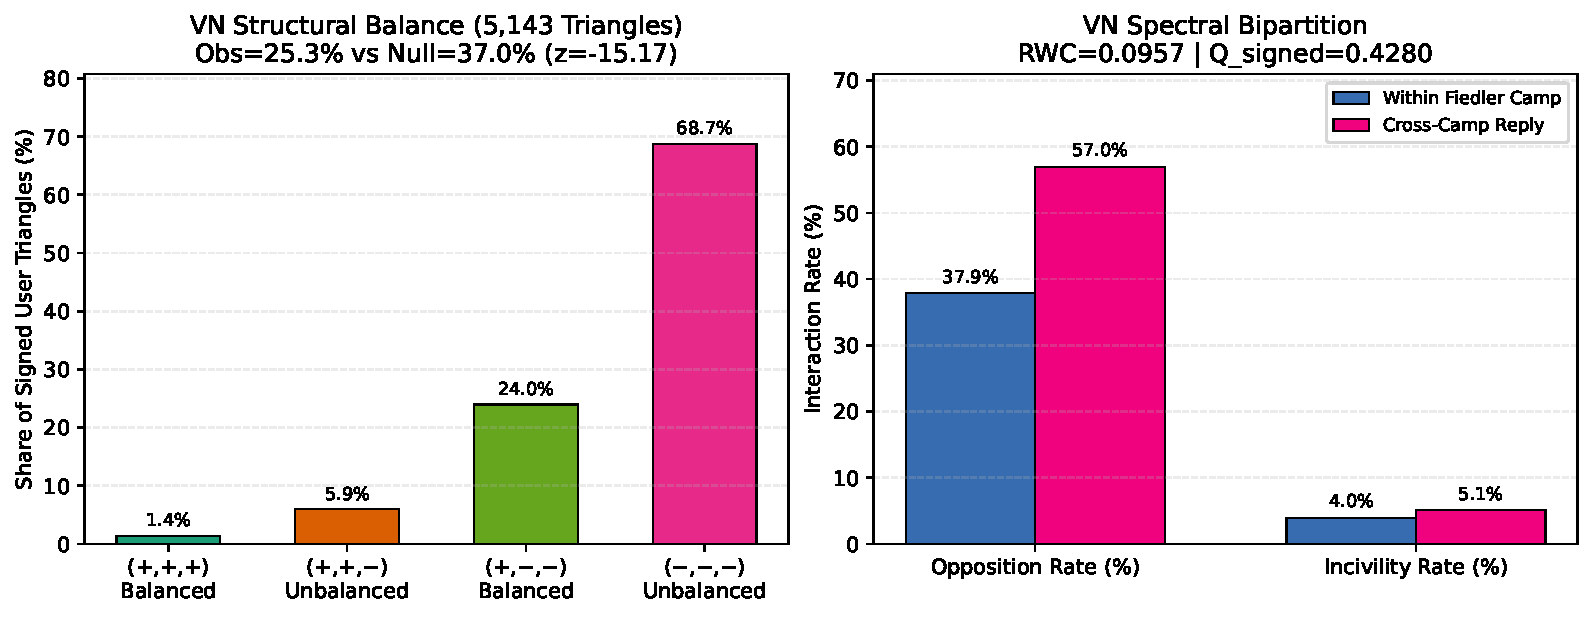
\includegraphics[width=\textwidth]{figures/vn/fig5_macro_signed_network.pdf}
\caption{Vietnamese Macro Signed User-Interaction Social Network ($13{,}718$ valid-pair users, $85{,}398$ interactions): Structural Balance triad distribution vs.\ uniform edge-sign permutation null ($z = -15.17$) and spectral two-camp opposition separation ($Q_{\text{signed}} = 0.4280$, $+19.1$~pp cross-camp conflict jump).}
\label{fig:macro_vn}
\end{figure*}
}{}

\IfFileExists{figures/pheme/fig5_macro_signed_network.pdf}{
\begin{figure*}[t]
\centering
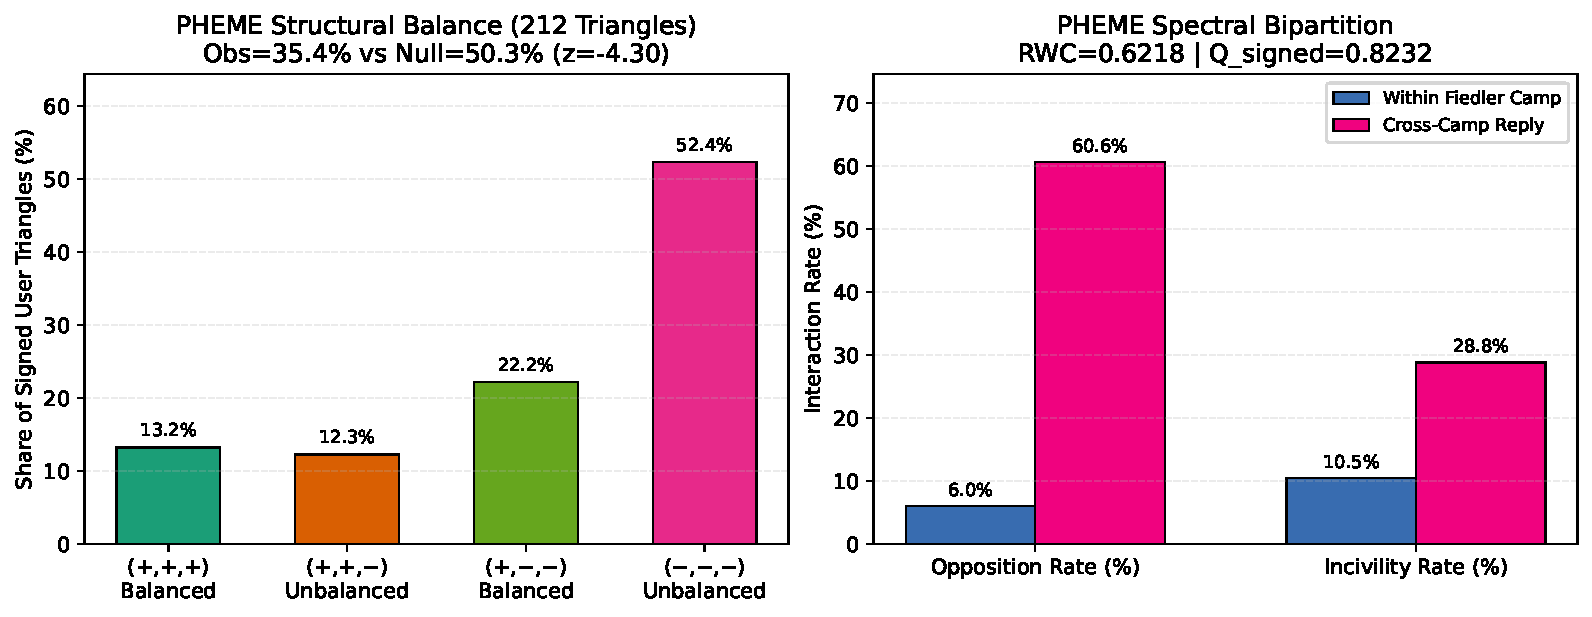
\includegraphics[width=\textwidth]{figures/pheme/fig5_macro_signed_network.pdf}
\caption{PHEME Macro Signed User-Interaction Social Network ($50{,}062$ total cohort users; $36{,}606$ valid-pair users; $72{,}858$ interactions; $10{,}364$-user WCC $= 20.7\%$ total / $28.3\%$ valid-pair): Structural Balance triad distribution ($35.4\%$ balanced across $212$ triangles, $z = -4.30$) and spectral two-camp separation ($Q_{\text{signed}} = 0.8232$, $+54.5$~pp cross-camp opposition jump, RWC $= 0.6218$).}
\label{fig:macro_pheme}
\end{figure*}
}{}

\subsection{English PHEME Reduced-Horizon Inductive and LOO Results}
On reduced-horizon PHEME ($K=10, N_{\text{reply}} \ge 15$, $334$ Test cascades; Table~\ref{tab:main_pheme}, with LOO Table~\ref{tab:loo_pheme} in Appendix~\ref{app:micro_ext} and UMAP Figure~\ref{fig:umap_pheme} in Appendix~\ref{app:diagnostics}), Early-$K$ Persistence collapses on polarization ($R^2_{\text{polar}} = -0.3022$, RMSE $= 0.0562$, $R^2_{\text{size}} = -0.0999$), whereas every learned model achieves positive $R^2_{\text{polar}} \in [0.0301, 0.0932]$. Inductively, \texttt{SBiFAGAT} attains the highest 4-class rumor \texttt{Macro-F1} ($0.3541 \pm 0.0261$, Holm--Bonferroni cascade-bootstrap $p_{\text{adj}} = 8.96\text{e-}02$, paired-$t$ $p_{\text{adj}} = 1.00$ vs.\ \texttt{EdgeGATv2} $0.3299$) and \texttt{Acc} $= 0.6359 \pm 0.0355$ (within-event cascade bootstrap $p_{\text{adj}} = 7.20\text{e-}03$ vs.\ \texttt{EdgeGATv2} $0.5988$, paired-$t$ $p_{\text{adj}} = 1.00$). On accuracy, \texttt{SBiFAGAT} trails \texttt{TemporalStanceMLP} ($0.6443 \pm 0.0267$) while exceeding the Test-334 \texttt{non-rumor} majority rate ($46.4\%$, $155/334$, compared to $68.2\%$ [$1{,}818/2{,}664$] across the full eligible cohort) by $+17.2$ percentage points. On regression, \texttt{SBiFAGAT} achieves $R^2_{\text{polar}} = 0.0793 \pm 0.0135$ (RMSE $= 0.0472 \pm 0.0003$, $r = 0.3755$, $\rho = 0.3888$) and MSLE $= 0.1007$ ($R^2_{\text{size}} = 0.0499$), trailing \texttt{TextMLP} on $R^2_{\text{polar}}$ ($0.0932$, RMSE $= 0.0469$) and \texttt{FAGCN} on size (MSLE $= 0.0986$, $R^2_{\text{size}} = 0.0697$). Under zero-shot $5$-fold LOO event shift with teacher-isolated edges (Table~\ref{tab:loo_pheme}), \texttt{SBiFAGAT} leads on \texttt{RMSE} ($0.0445 \pm 0.0028$), $R^2_{\text{polar}}$ ($0.0512 \pm 0.0317$), \texttt{Macro-F1} ($0.2978 \pm 0.0596$), and \texttt{Acc} ($0.6203 \pm 0.1443$ vs.\ \texttt{EdgeGATv2} $0.5874$ and \texttt{TextMLP} $0.6058$; Exact Perm.\ $p = 0.0625$ on \texttt{Acc}, $p_{\text{adj}} = 0.5625$), while trailing \texttt{Early-K Persistence} ($r = 0.3171, \rho = 0.3822$), \texttt{TemporalStanceMLP} ($0.2795 / 0.2891$), and \texttt{EdgeGATv2} ($0.2783 / 0.2783$) on polarization correlation ($r = 0.2739, \rho = 0.2737$) and closely trailing \texttt{EdgeGATv2} ($0.1594$) and \texttt{FAGCN} ($0.1596$) on size MSLE ($0.1600$).

\IfFileExists{tables_main_pheme.tex}{\begin{table*}[t]
\centering
\caption{English PHEME Early Cascade Size, Polarization, and Rumor Prediction at $K=10, N_{\text{reply}} \ge 15$ (Inductive, Mean $\pm$ Std, using Persistence Anchor and 8-D Burst Stats). Stars indicate fixed-seed cascade-level IID bootstrap significance across the 2 Test events vs.\ EdgeGATv2 ($^{*}p<0.05$, $^{**}p<0.01$; paired 5-seed $t$-test Holm--Bonferroni $p_{\text{adj}} = 1.00$).}
\label{tab:main_pheme}
\resizebox{\textwidth}{!}{
\begin{tabular}{lccccccccc}
\toprule
Model & MSLE $\downarrow$ & MAE $\downarrow$ & $R^2_{\text{size}}$ $\uparrow$ & RMSE $\downarrow$ & $R^2_{\text{polar}}$ $\uparrow$ & Pearson $r$ $\uparrow$ & Spearman $\rho$ $\uparrow$ & Macro-F1 $\uparrow$ & Acc $\uparrow$ \\
\midrule
Early-K Persistence & 0.1166 $\pm$ 0.0000 & 0.2821 $\pm$ 0.0000 & -0.0999 $\pm$ 0.0000 & 0.0562 $\pm$ 0.0000 & -0.3022 $\pm$ 0.0000 & 0.3310 $\pm$ 0.0000 & 0.3951 $\pm$ 0.0000 & -- & -- \\
TextMLP & 0.1002 $\pm$ 0.0066 & 0.2486 $\pm$ 0.0236 & 0.0545 $\pm$ 0.0620 & \textbf{0.0469 $\pm$ 0.0004} & \textbf{0.0932 $\pm$ 0.0162} & 0.3640 $\pm$ 0.0369 & 0.3893 $\pm$ 0.0657 & 0.3379 $\pm$ 0.0202 & 0.6228 $\pm$ 0.0500 \\
TemporalStanceMLP & 0.1006 $\pm$ 0.0055 & 0.2371 $\pm$ 0.0219 & 0.0509 $\pm$ 0.0514 & 0.0470 $\pm$ 0.0012 & 0.0861 $\pm$ 0.0460 & 0.3739 $\pm$ 0.0400 & 0.4091 $\pm$ 0.0419 & 0.3440 $\pm$ 0.0187 & \textbf{0.6443 $\pm$ 0.0267} \\
StandardGCN & 0.1003 $\pm$ 0.0038 & 0.2448 $\pm$ 0.0131 & 0.0538 $\pm$ 0.0354 & 0.0478 $\pm$ 0.0004 & 0.0586 $\pm$ 0.0165 & 0.3033 $\pm$ 0.0537 & 0.3326 $\pm$ 0.0749 & 0.3195 $\pm$ 0.0219 & 0.5790 $\pm$ 0.0733 \\
StandardGATv2 & 0.0998 $\pm$ 0.0068 & 0.2446 $\pm$ 0.0230 & 0.0585 $\pm$ 0.0638 & 0.0475 $\pm$ 0.0003 & 0.0679 $\pm$ 0.0124 & 0.3115 $\pm$ 0.0125 & 0.3210 $\pm$ 0.0418 & 0.3263 $\pm$ 0.0433 & 0.6210 $\pm$ 0.0547 \\
EdgeGATv2 & 0.0996 $\pm$ 0.0072 & 0.2410 $\pm$ 0.0220 & 0.0609 $\pm$ 0.0675 & 0.0472 $\pm$ 0.0007 & 0.0803 $\pm$ 0.0260 & \textbf{0.4008 $\pm$ 0.0472} & \textbf{0.4451 $\pm$ 0.0307} & 0.3299 $\pm$ 0.0522 & 0.5988 $\pm$ 0.0988 \\
FAGCN & \textbf{0.0986 $\pm$ 0.0062} & \textbf{0.2329 $\pm$ 0.0161} & \textbf{0.0697 $\pm$ 0.0584} & 0.0485 $\pm$ 0.0007 & 0.0301 $\pm$ 0.0268 & 0.3171 $\pm$ 0.0589 & 0.3467 $\pm$ 0.0915 & 0.3238 $\pm$ 0.0262 & 0.5605 $\pm$ 0.0221 \\
BiGCN & 0.1066 $\pm$ 0.0086 & 0.2592 $\pm$ 0.0220 & -0.0054 $\pm$ 0.0813 & 0.0482 $\pm$ 0.0008 & 0.0408 $\pm$ 0.0329 & 0.2830 $\pm$ 0.0475 & 0.2833 $\pm$ 0.0633 & 0.2674 $\pm$ 0.1028 & 0.5563 $\pm$ 0.0939 \\
SBiFAGAT & 0.1007 $\pm$ 0.0061 & 0.2424 $\pm$ 0.0210 & 0.0499 $\pm$ 0.0575 & 0.0472 $\pm$ 0.0003 & 0.0793 $\pm$ 0.0135 & 0.3755 $\pm$ 0.0505 & 0.3888 $\pm$ 0.0678 & \textbf{0.3541 $\pm$ 0.0261} & 0.6359 $\pm$ 0.0355$^{**}$ \\
\midrule
$p$-value (SBiFAGAT vs. EdgeGATv2) & 4.92e-01 & 7.93e-01 & 4.92e-01 & 9.45e-01 & 9.50e-01 & 4.65e-01 & 1.64e-01 & 3.82e-01 & 3.00e-01 \\
Bootstrap $p$ (SBiFAGAT vs. EdgeGATv2) & 4.34e-01 & 4.02e-01 & 4.31e-01 & 8.32e-01 & 8.48e-01 & 1.25e-01 & 7.20e-03 & 1.28e-02 & 8.00e-04 \\
Holm-Bonferroni $p$ (SBiFAGAT vs. EdgeGATv2) & 1.00e+00 & 1.00e+00 & 1.00e+00 & 1.00e+00 & 1.00e+00 & 1.00e+00 & 1.00e+00 & 1.00e+00 & 1.00e+00 \\
Holm-Bonf Bootstrap $p$ (SBiFAGAT vs. EdgeGATv2) & 1.00e+00 & 1.00e+00 & 1.00e+00 & 1.00e+00 & 1.00e+00 & 7.49e-01 & 5.76e-02 & 8.96e-02 & 7.20e-03 \\
\bottomrule
\end{tabular}
}
\end{table*}
}{}

\subsection{Component Ablation and Early-Horizon Sensitivity}
On the Vietnamese component ablation (Table~\ref{tab:ablation_vn} in Appendix~\ref{app:micro_ext}), \texttt{SBiFAGAT (Full)} achieves $R^2_{\text{polar}} = 0.0777 \pm 0.0141$ and $R^2_{\text{size}} = 0.2925 \pm 0.0315$, statistically tied with matched \texttt{BiEdgeGATv2} ($R^2_{\text{polar}} = 0.0789$, $R^2_{\text{size}} = 0.2962$, $\rho = 0.2530$; Holm--Bonferroni $p_{\text{adj}} = 1.00$). Ablating Camp Dipole \& Moments ($R^2_{\text{polar}} = 0.0503$) or replacing the signed Conflict Gate with an unsigned sigmoid ($0.0527$) causes the largest drops in polarization explained variance, while removing $c_{\mathcal{G}}$ drops $R^2_{\text{size}}$ from $0.2925$ to $0.2215$; removing $h_{uv}$ leaves VN polarization nearly unchanged ($0.0757$). Minor metric differences between Table~\ref{tab:main_vn} ($0.0742$) and Table~\ref{tab:ablation_vn} ($0.0777$) stem from CUDA non-deterministic \texttt{scatter\_add}/\texttt{atomicAdd} reductions across separate Kaggle GPU sessions (all runs reseed deterministically prior to each model).

In contrast, on reduced-horizon PHEME ($K=10$, Table~\ref{tab:ablation_pheme} in Appendix~\ref{app:micro_ext}), \texttt{SBiFAGAT (Full)} wins $0/9$ metrics: $8/11$ component ablations plus \texttt{BiEdgeGATv2 (Matched)} ($9/12$ non-Full rows) exceed \texttt{Full} ($R^2_{\text{polar}} = 0.0791$; minor Table~\ref{tab:main_pheme} vs.\ Table~\ref{tab:ablation_pheme} differences---e.g., $0.0793$ vs.\ $0.0791$ $R^2_{\text{polar}}$ and $0.6359$ vs.\ $0.6383$ \texttt{Acc}---reflect cross-session CUDA non-deterministic \texttt{scatter\_add}/\texttt{atomicAdd} reductions), led by \texttt{w/o Burst Stats} ($0.1015$), \texttt{w/o Dir-GNN Mixing} ($0.1010$, also leading \texttt{MSLE} $= 0.0985$, \texttt{MAE} $= 0.2344$, $R^2_{\text{size}} = 0.0712$, and $\rho = 0.4408$), \texttt{w/o Bottom-Up} ($0.1009$, leading $r = 0.4058$), \texttt{w/o Camp Dipole \& Moments} ($0.0964$), and \texttt{w/o Edge Signals} (leading \texttt{Macro-F1} $= 0.3580$). Moreover, \texttt{BiEdgeGATv2 (Matched)} significantly outperforms \texttt{SBiFAGAT (Full)} across all four polarization metrics under cascade-level bootstrap (\texttt{RMSE} $0.0469$ vs.\ $0.0472$, $p_{\text{adj}} = 7.20\text{e-}03$; $R^2_{\text{polar}} = 0.0940$ vs.\ $0.0791$, $p_{\text{adj}} = 8.00\text{e-}03$; $r = 0.4026$ vs.\ $0.3754$, $p_{\text{adj}} = 2.88\text{e-}02$; $\rho = 0.4338$ vs.\ $0.3892$, $p_{\text{adj}} = 7.20\text{e-}03$; paired-$t$ $p_{\text{adj}} = 1.00$), whereas the table's one-sided star rule marks only \texttt{SBiFAGAT}'s bootstrap lead on \texttt{Macro-F1} ($0.3553$ vs.\ $0.3312$) and \texttt{Acc} ($0.6383$ vs.\ $0.6138$, $p_{\text{adj}} = 7.20\text{e-}03$). Although removing the Persistence Anchor ($0.0653$), all edge signals ($0.0676$), or stance $s_{uv}$ ($0.0710$) still degrades $R^2_{\text{polar}}$ relative to \texttt{Full}, simplifying multi-layer directional message passing consistently improves polarization regression on $11$-node PHEME trees. Across $K \in \{10, 20, 30, 50\}$ on fixed-future subsets ($N_{\text{reply}} \ge 55$, evaluating unobserved future replies strictly past reply index $k > 50$; Figures~\ref{fig:k_curve_vn} and~\ref{fig:k_curve_pheme} in Appendix~\ref{app:diagnostics}), VN size MSLE tightens steadily from $0.1443$ ($K=10$) and $0.1370$ ($K=20$) to $0.1352$ ($K=30$) and $0.1053$ ($K=50$, vs.\ \texttt{StandardGCN} $0.0995$). On the small $n=10$ PHEME $K$-curve subset, although \texttt{SBiFAGAT} reduces MSLE from $0.0893$ ($K=10$) to $0.0612$ ($K=50$) and raises $r$ from $0.0647$ to $0.2349$, $R^2_{\text{size}}$ remains negative at every horizon ($-0.9883$ at $K=10$ to $-0.3621$ at $K=50$) and 4-class rumor prediction collapses completely to predicting the majority \texttt{non-rumor} class across all five seeds (\texttt{Acc} $= 0.7000 \pm 0.0000$, \texttt{Macro-F1} $= 0.2745 \pm 0.0000$).

\subsection{Post-Hoc Text-Free UPFD Structural Transfer}
Tables~\ref{tab:upfd_results} and~\ref{tab:upfd_politifact} (Appendix~\ref{app:transfer_audit}) report post-hoc text-free fake-news detection on PyG UPFD (BERT 768-d node embeddings with learned latent edges). On GossipCop, \texttt{StandardGATv2} ($0.9684 \pm 0.0032$ accuracy; \texttt{ROC-AUC} $= 0.9929$) and \texttt{EdgeGATv2 (Latent)} ($0.9682$; \texttt{ROC-AUC} $= 0.9937$) significantly outperform \texttt{SBiFAGAT (Latent)} ($0.9486 \pm 0.0077$; \texttt{ROC-AUC} $= 0.9859$; Holm--Bonferroni bootstrap $p_{\text{adj}} = 8.00\text{e-}04$, paired-$t$ $p_{\text{adj}} = 1.30\text{e-}02$), showing that latent stance gating adds no benefit when reply texts and real conflict labels are absent. On smaller PolitiFact, \texttt{EdgeGATv2 (Latent)} ($0.8253 \pm 0.0099$ accuracy, $0.8251 \pm 0.0101$ \texttt{Macro-F1}, $0.8775$ \texttt{ROC-AUC}) outperforms \texttt{SBiFAGAT (Latent)} ($0.8090 \pm 0.0240$ accuracy, $0.8083 \pm 0.0249$ \texttt{Macro-F1}, $0.8627$ \texttt{ROC-AUC}; Holm--Bonferroni bootstrap $p_{\text{adj}} = 3.20\text{e-}02$, paired-$t$ $p_{\text{adj}} = 0.2660$), while both edge-latent models exhibit substantially lower seed variance than \texttt{StandardGCN} ($0.8063 \pm 0.1650$) and \texttt{StandardGATv2} ($0.7701 \pm 0.1450$).

\subsection{Reliability, Construct Alignment, Sensitivity, and Efficiency}\label{sec:reliability}
\textbf{Silver-Label Construct Validity \& Verified-Gold Audits:} Early-graph construct correlations remain weak on shallow early trees (Spearman Sarle's BC correlation $= -0.0152$ and signed assortativity correlation $= -0.0589$ on VN; $0.0800$ and $-0.1136$ on PHEME). On SemEval-2019 RumourEval Test ($1{,}675$ pairs), $476$ replies ($28.4\%$) lie at depth $\ge 2$ where direct parent context diverges from root context (e.g., affirming the root claim while negating a skeptical parent); evaluating both protocols yields higher stance \texttt{Macro-F1} in root-context mode ($0.3311$, \texttt{Acc} $= 0.8179$, $\kappa = -0.0149$, $\rho = 0.0917$) than parent-context mode ($0.3270$, \texttt{Acc} $= 0.8185$, $\kappa = -0.0172$). However, zero-shot \texttt{mDeBERTa-v3-xnli} routes $93.0\%$ ($1{,}557/1{,}675$ under root context) of replies to \texttt{neutral}, causing accuracy ($81.8\%$) to fall below the $87.8\%$ ($1{,}471/1{,}675$ \texttt{query+comment}) \texttt{neutral} majority baseline and yielding class recall of only $3.8\%$ ($4/104$) on \texttt{support} and $3.0\%$ ($3/100$, root) / $2.0\%$ ($2/100$, parent) on \texttt{oppose}. On VN, blind audits used LLM-assisted pre-annotation (\texttt{Gemini Flash-Lite}) verified by a single author (single-author verified gold, \texttt{IAA} $= \text{--}$; Table~\ref{tab:human_audit} in Appendix~\ref{app:transfer_audit}). The $20$-pair pilot yields stance \texttt{Macro-F1} $= 0.6640$ (\texttt{Acc} $= 70.0\%$, weighted accuracy $64.78\%$, $\kappa = 0.5420$, $\rho = 0.5856$) and hostility \texttt{ROC-AUC} $= 1.0000$ (\texttt{Acc} $= 75.0\%$). On the $120$-pair Test audit, unweighted stance alignment drops to \texttt{Macro-F1} $= 0.3760$ (\texttt{Acc} $= 40.0\%$, $\kappa = 0.1000$, $\rho = 0.2726$), while inverse-sampling-weighted population metrics drop to weighted accuracy $= 24.79\%$ and weighted \texttt{Macro-F1} $= 0.2324$ (below $33.3\%$ 3-class chance). For VN $N=120$ hostility discrimination, \texttt{uitnlp/visobert} achieves \texttt{ROC-AUC} $= 0.9841$, \texttt{PR-AUC} $= 0.2619$, $\rho = 0.3543$, $\kappa = 0.2475$, unweighted \texttt{Acc} $= 69.17\%$ (weighted accuracy $96.63\%$), and overall \texttt{Macro-F1} $= 0.5743$ (weighted \texttt{Macro-F1} $= 0.6641$), while positive-class (\texttt{uncivil}) performance is precision $= 0.2128$ ($10/47$), recall $= 1.00$ ($10/10$), and positive-class \texttt{F1} $= 0.3509$. Across $30$ verified VN Test trees, empirical future $y_{\text{polar}} \in [0.0447, 0.2644]$ yields near-random alignment with 0--4 perceived division ($r = 0.0284, \rho = 0.0018, \tau_b = 0.0026, \kappa_w = 0.0192$, \texttt{ROC-AUC} at grade $\ge 2 = 0.5402$) because polite binary-choice advice threads raise $m_+ m_-$, whereas shared-target outrage threads pull replies uniformly to one side. Accordingly, Tier~1 regression should be interpreted strictly as modeling NLI-derived stance dispersion rather than human-perceived division.

\textbf{Target-Misattributed Profanity Diagnosis:} Across all $86{,}320$ VN edges, hostility correlates negatively with stance polarity ($r = -0.1832$); among $3{,}597$ ($4.17\%$) uncivil edges ($h_{uv} \ge 0.5$), $62.97\%$ receive $s_{uv} < -0.15$ vs.\ only $1.14\%$ ($41$) receiving $s_{uv} > 0.15$. Auditing the combined $N = 140$ VN pairs ($20$ pilot $+$ $120$ Test) exposes \emph{Target-Misattributed Profanity}: the NLI teacher flips $4/7$ ($57.1\%$) \texttt{support+uncivil} replies---where commenters curse a third party in solidarity with the parent---into negative opposition (mean $s_{uv} = -0.2495$, more negative than \texttt{oppose+clean} at $-0.1594$). Because fine-tuned \texttt{uitnlp/visobert} captures target-agnostic utterance incivility without target attribution (on $N=140$ at threshold $0.5$: \texttt{Acc} $= 70.0\%$, recall $= 1.00$, precision $= 0.2075$ [$11/53$], positive-class \texttt{F1} $= 0.3438$), removing $h_{uv}$ leaves VN $R^2_{\text{polar}}$ nearly unchanged ($0.0777 \to 0.0757$) and raises PHEME $R^2_{\text{polar}}$ ($0.0791 \to 0.0878$), confirming three-class stance as the core edge signal.

\textbf{Interpretability, Sensitivity, and Cost:} Figures~\ref{fig:heatmap_vn} and~\ref{fig:heatmap_pheme} (Appendix~\ref{app:diagnostics}) visualize top trigger replies ranked by $|\gamma|$. In observational edge-sensitivity analysis (Tables~\ref{tab:mechanisms_vn} and~\ref{tab:mechanisms_pheme}; Figures~\ref{fig:cf_vn} and~\ref{fig:cf_pheme} in Appendix~\ref{app:diagnostics}), cascades are partitioned into \emph{hostile conflict} (mean early hostility $\bar{h} \ge 0.25$), \emph{civil disagreement} (otherwise fraction of early edges with $s_{uv} < -0.15$ at least $0.20$), and \emph{low conflict} (remainder); early hostility correlates positively with cascade size on both VN ($\rho = 0.2128, r = 0.2044$; $149$ civil disagreement, $75$ low conflict, $1$ hostile conflict across $225$ Test threads) and PHEME ($\rho = 0.2024, r = 0.1901$; $204$ low conflict, $9$ civil disagreement, $121$ hostile conflict across $334$ Test threads), while early stance dispersion correlates with future polarization (VN $r = 0.1593$; PHEME $r = 0.2656, \rho = 0.3198$). Cooling all early hostility yields small linear shifts in predicted size (VN $\Delta\hat{y}_{\text{size}} = +0.0024$; PHEME $-0.0052$), whereas neutralizing top-3 triggers shifts $\Delta\hat{y}_{\text{polar}}$ negatively (VN $-0.0007$; PHEME $-0.0011$). Efficiency profiling (Table~\ref{tab:efficiency} in Appendix~\ref{app:transfer_audit}) shows \texttt{SBiFAGAT} uses $137{,}086$ parameters and $1.1721$~ms/cascade ($0.03$~MB peak allocated CPU RAM; $27.09$~MB peak CUDA VRAM on PHEME) vs.\ $71{,}110$ parameters and $0.0787$~ms/cascade ($21.08$~MB peak VRAM) for \texttt{TextMLP}.

\section{Limitations, Future Work, and Ethical Safeguards}
We explicitly acknowledge five methodological constraints:
\begin{enumerate}
    \item \textbf{Early Tree Ceiling vs.\ Macro Network Nuances:} Micro early trees ($|\mathcal{V}_K| \le 21$ on VN, $|\mathcal{V}_K| \le 11$ on PHEME) are text-dominated, explaining why \texttt{SBiFAGAT} ties \texttt{TextMLP}/\texttt{BiEdgeGATv2} on VN polarization, wins $0/9$ PHEME ablation metrics (trailing \texttt{BiEdgeGATv2} on polarization $0.0791$ vs.\ $0.0940$), and yields negative $R^2_{\text{size}}$ and majority-class collapse on the $n=10$ PHEME $K$-curve. On Tier~2 macro networks, both corpora are anti-balanced ($(---)$ triads, $z = -15.17 / -4.30$) and the PHEME WCC is sparse ($212$ triangles); moreover, chronological link evaluation leaves Train pairs unmasked during Val/Test message passing ($21.7\%$ PHEME / $3.2\%$ VN transductive recurring-pair overlap), retains pre-cutoff neutral/sub-threshold features for $6.6\%$--$10.1\%$ of unseen users, and supplies continuous 2D edges only to \texttt{SBiFAGAT-Link}.
    \item \textbf{Silver-Label Collapse and Target-Misattributed Profanity:} Early $y_{\text{polar}}^{\text{early}}$ runs BFS propagation over Student edges without direct $(\text{root}, \text{reply})$ overrides, whereas future $y_{\text{polar}}$ uses Teacher edges with direct $(\text{root}, \text{reply})$ predictions when available (Temporal/LOO protocols isolate inputs using Teacher edges). VN audits reflect AI-pre-annotated (\texttt{Gemini Flash-Lite}) single-author verification (\texttt{IAA} $= \text{--}$), weak weighted stance alignment ($24.79\%$), near-random tree correlation ($\rho = 0.0018$), RumourEval minority recall collapse ($2.0\%$--$3.8\%$; $81.8\%$ vs.\ $87.8\%$ majority), and $57.1\%$ \texttt{support+uncivil} NLI flips.
    \item \textbf{Heuristic VN Topics and Horizon Cohort Size:} VN Reddit is $99.96\%$ \texttt{r/vozforums} (\texttt{r/VietNam} $32$ nodes) and yields $1{,}496/1{,}500$ singleton clusters under 30-day TF-IDF grouping, while reduced-horizon PHEME ($K=10, N_{\text{reply}} \ge 15$) evaluates $334$ inductive Test trees across only $2$ Test events ($10$ trees in the $N_{\text{reply}} \ge 55$ $K$-curve) and $5$ LOO event folds.
    \item \textbf{Audit Sampling and Observational Sensitivity:} Tree audits display up to $12$ evenly spaced future replies against empirical quintile grades; Section~\ref{sec:reliability} perturbations probe model linearity rather than causal moderation effects.
    \item \textbf{Privacy Protection:} All user identifiers undergo secret-salted SHA-256 pseudonymization, PII and crypto spam are automatically filtered prior to persistence, and sealed machine keys are excluded from public artifacts.
\end{enumerate}

\textbf{Future Work:} Three directions directly address these failure modes: (i) \emph{Target-Aware Stance Modeling}, replacing target-agnostic zero-shot NLI and utterance-level hostility with target-conditioned stance/toxicity architectures to eliminate \emph{Target-Misattributed Profanity} ($57.1\%$ third-party-cursing flip rate); (ii) \emph{Multi-Turn Thread Context ($\ge 5$ turns)}, expanding beyond the 2-turn \texttt{[CLS] root [SEP] parent [SEP] reply [SEP]} horizon to encode $\ge 5$ ancestor turns (grandparents and higher conversational context) for resolving multi-hop negation and sarcasm; and (iii) \emph{Reply-Mention Heterogeneous Graphs \& Scalable Ingestion}, integrating explicit \texttt{@mention} edges alongside reply edges and paginating live Reddit ingestion past the single-request $500$-comment API limit.

\section{Conclusion}
We presented an Extended Technical Report for a leakage-checked two-tier signed GNN and NLP framework spanning early-cascade size, polarization, and rumor veracity forecasting (\texttt{SBi-FAGAT}) alongside macro cross-thread user-interaction polarization and chronological signed link prediction. Controlled five-seed experiments establish an honest empirical boundary across scales: on shallow early cascades, \texttt{SBiFAGAT} clearly surpasses Early-$K$ Persistence ($-3.1986 \to 0.0742$ on VN; $-0.3022 \to 0.0793$ on PHEME), achieves the highest inductive PHEME rumor \texttt{Macro-F1} ($0.3541$, bootstrap $p_{\text{adj}} = 8.96\text{e-}02$) and \texttt{Acc} $= 0.6359$ (bootstrap $p_{\text{adj}} = 7.20\text{e-}03$ vs.\ \texttt{EdgeGATv2}, $+17.2$~pp above Test-334 majority while trailing \texttt{TemporalStanceMLP} at $0.6443$), and leads PHEME $5$-fold LOO on RMSE ($0.0445$), $R^2_{\text{polar}}$ ($0.0512$), \texttt{Macro-F1} ($0.2978$), and \texttt{Acc} ($0.6203$) while trailing \texttt{Early-K Persistence} and \texttt{EdgeGATv2} on correlation ($r/\rho$). At the same time, ablations and audits reveal clear structural limits on shallow $11$--$21$-node trees---\texttt{SBiFAGAT} ties regular text/edge baselines on VN, wins $0/9$ metrics in PHEME ablation (trailing \texttt{BiEdgeGATv2} on $R^2_{\text{polar}}$), and suffers from NLI \emph{Target-Misattributed Profanity} ($57.1\%$). Conversely, projecting the same 2D discourse attributes onto macro user networks exposes pronounced spectral two-camp separation (VN $Q_{\text{signed}} = 0.4280$, $+19.1$~pp cross-camp opposition, anti-balanced $z = -15.17$; PHEME $Q_{\text{signed}} = 0.8232$ on a sparse $212$-triangle WCC, $+54.5$~pp, RWC $= 0.6218$, $z = -4.30$), where \texttt{SBiFAGAT-Link} yields directional transductive gains on PHEME (\texttt{ROC-AUC} $= 0.9181$, \texttt{Macro-F1} $= 0.8006$; $p_{\text{adj}} = 0.1622 / 0.3750$, $21.7\%$ recurring-pair overlap).

\bibliographystyle{IEEEtran}
\bibliography{references}

\clearpage
\appendices
\section{Extended Benchmarks, Audits, and Diagnostic Probes}\label{app:extended}
\subsection{Extended Micro-Cascade Benchmarks and Ablations}\label{app:micro_ext}
Tables~\ref{tab:temporal_vn}--\ref{tab:ablation_pheme} provide the complete five-seed results for VN chronological temporal holdout (Table~\ref{tab:temporal_vn}), PHEME $5$-fold LOO event-shift evaluation (Table~\ref{tab:loo_pheme}), and full component ablations on VN (Table~\ref{tab:ablation_vn}) and reduced-horizon PHEME (Table~\ref{tab:ablation_pheme}).

\subsection{External Transfer, Human Audits, and Efficiency}\label{app:transfer_audit}
Tables~\ref{tab:upfd_results}--\ref{tab:efficiency} present post-hoc text-free UPFD transfer on GossipCop and PolitiFact (Tables~\ref{tab:upfd_results}--\ref{tab:upfd_politifact}), VN verified-gold and RumourEval-2019 SDQC stance audits (Table~\ref{tab:human_audit}), and model parameter/latency/memory profiling (Table~\ref{tab:efficiency}).

\subsection{Diagnostic Visualizations and Sensitivity Probes}\label{app:diagnostics}
Figures~\ref{fig:umap_vn}--\ref{fig:cf_pheme} and Tables~\ref{tab:mechanisms_vn}--\ref{tab:mechanisms_pheme} collect UMAP node projections (Figures~\ref{fig:umap_vn}--\ref{fig:umap_pheme}), early $K$-horizon sensitivity curves (Figures~\ref{fig:k_curve_vn}--\ref{fig:k_curve_pheme}), gate heatmaps (Figures~\ref{fig:heatmap_vn}--\ref{fig:heatmap_pheme}), and observational edge-feature sensitivity probes (Figures~\ref{fig:cf_vn}--\ref{fig:cf_pheme}; Tables~\ref{tab:mechanisms_vn}--\ref{tab:mechanisms_pheme}).

\IfFileExists{tables_temporal_vn.tex}{\begin{table*}[t]
\centering
\caption{Early Cascade Size and Future Polarization Forecasting at $K=20$ (TEMPORAL, Mean $\pm$ Std). Stars indicate significance vs. TemporalStanceMLP ($^{*}p<0.05$, $^{**}p<0.01$).}
\label{tab:temporal_vn}
\resizebox{\textwidth}{!}{
\begin{tabular}{lccccccc}
\toprule
Model & MSLE $\downarrow$ & MAE $\downarrow$ & $R^2_{\text{size}}$ $\uparrow$ & RMSE $\downarrow$ & $R^2_{\text{polar}}$ $\uparrow$ & Pearson $r$ $\uparrow$ & Spearman $\rho$ $\uparrow$ \\
\midrule
Early-K Persistence & 0.2540 $\pm$ 0.0000 & 0.4041 $\pm$ 0.0000 & -0.0013 $\pm$ 0.0000 & 0.0874 $\pm$ 0.0000 & -5.4386 $\pm$ 0.0000 & 0.1778 $\pm$ 0.0000 & 0.1741 $\pm$ 0.0000 \\
TextMLP & 0.2015 $\pm$ 0.0105 & 0.3448 $\pm$ 0.0101 & 0.2058 $\pm$ 0.0415 & 0.0332 $\pm$ 0.0006 & 0.0702 $\pm$ 0.0333 & 0.3267 $\pm$ 0.0282 & 0.2938 $\pm$ 0.0274 \\
TemporalStanceMLP & 0.2003 $\pm$ 0.0059 & 0.3420 $\pm$ 0.0066 & 0.2103 $\pm$ 0.0232 & \textbf{0.0330 $\pm$ 0.0004} & \textbf{0.0815 $\pm$ 0.0198} & \textbf{0.3377 $\pm$ 0.0112} & 0.2875 $\pm$ 0.0276 \\
StandardGCN & 0.1972 $\pm$ 0.0080 & 0.3353 $\pm$ 0.0064 & 0.2227 $\pm$ 0.0315 & 0.0330 $\pm$ 0.0003 & 0.0815 $\pm$ 0.0167 & 0.3289 $\pm$ 0.0190 & 0.3034 $\pm$ 0.0077 \\
StandardGATv2 & 0.1996 $\pm$ 0.0053 & 0.3362 $\pm$ 0.0090 & 0.2134 $\pm$ 0.0210 & 0.0334 $\pm$ 0.0008 & 0.0598 $\pm$ 0.0462 & 0.3244 $\pm$ 0.0386 & 0.2983 $\pm$ 0.0303 \\
EdgeGATv2 & 0.1971 $\pm$ 0.0065 & 0.3397 $\pm$ 0.0082 & 0.2230 $\pm$ 0.0257 & 0.0331 $\pm$ 0.0003 & 0.0765 $\pm$ 0.0162 & 0.3312 $\pm$ 0.0159 & 0.2846 $\pm$ 0.0165 \\
FAGCN & \textbf{0.1881 $\pm$ 0.0129} & \textbf{0.3298 $\pm$ 0.0133} & \textbf{0.2586 $\pm$ 0.0509} & 0.0333 $\pm$ 0.0003 & 0.0664 $\pm$ 0.0176 & 0.3266 $\pm$ 0.0217 & 0.2887 $\pm$ 0.0231 \\
BiGCN & 0.2021 $\pm$ 0.0079 & 0.3446 $\pm$ 0.0115 & 0.2033 $\pm$ 0.0310 & 0.0336 $\pm$ 0.0002 & 0.0481 $\pm$ 0.0129 & 0.2930 $\pm$ 0.0194 & 0.2675 $\pm$ 0.0282 \\
SBiFAGAT & 0.2051 $\pm$ 0.0126 & 0.3461 $\pm$ 0.0070 & 0.1914 $\pm$ 0.0495 & 0.0334 $\pm$ 0.0009 & 0.0609 $\pm$ 0.0491 & 0.3338 $\pm$ 0.0319 & \textbf{0.3058 $\pm$ 0.0187} \\
\midrule
$p$-value (SBiFAGAT vs. TemporalStanceMLP) & 3.11e-01 & 1.89e-01 & 3.11e-01 & 4.36e-01 & 4.31e-01 & 8.28e-01 & 3.10e-01 \\
Bootstrap $p$ (SBiFAGAT vs. TemporalStanceMLP) & 1.40e-01 & 2.16e-01 & 1.34e-01 & 2.61e-01 & 2.42e-01 & 8.95e-01 & 2.13e-01 \\
Holm-Bonferroni $p$ (SBiFAGAT vs. TemporalStanceMLP) & 1.00e+00 & 1.00e+00 & 1.00e+00 & 1.00e+00 & 1.00e+00 & 1.00e+00 & 1.00e+00 \\
Holm-Bonf Bootstrap $p$ (SBiFAGAT vs. TemporalStanceMLP) & 9.35e-01 & 1.00e+00 & 9.35e-01 & 1.00e+00 & 1.00e+00 & 1.00e+00 & 1.00e+00 \\
\bottomrule
\end{tabular}
}
\end{table*}
}{}
\IfFileExists{tables_loo_pheme.tex}{\begin{table*}[t]
\centering
\caption{English PHEME 5-Fold Leave-One-Event-Out (LOO) Early Cascade Size, Polarization, and Rumor Prediction at $K=10, N_{\text{reply}} \ge 15$ (Teacher-Isolated Edges, Mean $\pm$ Std, using Persistence Anchor and 8-D Burst Stats). Stars indicate significance vs.\ EdgeGATv2 ($^{*}p<0.05$, $^{**}p<0.01$; Exact Perm.\ Holm--Bonferroni $p_{\text{adj}} \ge 0.5625$).}
\label{tab:loo_pheme}
\resizebox{\textwidth}{!}{
\begin{tabular}{lccccccccc}
\toprule
Model & MSLE $\downarrow$ & MAE $\downarrow$ & $R^2_{\text{size}}$ $\uparrow$ & RMSE $\downarrow$ & $R^2_{\text{polar}}$ $\uparrow$ & Pearson $r$ $\uparrow$ & Spearman $\rho$ $\uparrow$ & Macro-F1 $\uparrow$ & Acc $\uparrow$ \\
\midrule
Early-K Persistence & 0.1767 $\pm$ 0.0919 & 0.3133 $\pm$ 0.0757 & -0.0602 $\pm$ 0.0719 & 0.0577 $\pm$ 0.0080 & -0.6127 $\pm$ 0.3867 & \textbf{0.3171 $\pm$ 0.0889} & \textbf{0.3822 $\pm$ 0.0565} & -- & -- \\
TextMLP & 0.1613 $\pm$ 0.0836 & 0.2836 $\pm$ 0.0746 & 0.0233 $\pm$ 0.1147 & 0.0450 $\pm$ 0.0028 & 0.0316 $\pm$ 0.0183 & 0.2404 $\pm$ 0.0673 & 0.2353 $\pm$ 0.0823 & 0.2910 $\pm$ 0.0479 & 0.6058 $\pm$ 0.1481 \\
TemporalStanceMLP & 0.1610 $\pm$ 0.0827 & \textbf{0.2822 $\pm$ 0.0735} & 0.0294 $\pm$ 0.0899 & 0.0447 $\pm$ 0.0027 & 0.0432 $\pm$ 0.0241 & 0.2795 $\pm$ 0.0606 & 0.2891 $\pm$ 0.0702 & 0.2655 $\pm$ 0.0461 & 0.5719 $\pm$ 0.1531 \\
StandardGCN & 0.1600 $\pm$ 0.0842 & 0.2830 $\pm$ 0.0753 & 0.0372 $\pm$ 0.0901 & 0.0455 $\pm$ 0.0033 & 0.0103 $\pm$ 0.0285 & 0.2141 $\pm$ 0.0619 & 0.2050 $\pm$ 0.0982 & 0.2740 $\pm$ 0.0551 & 0.5908 $\pm$ 0.1722 \\
StandardGATv2 & 0.1613 $\pm$ 0.0831 & 0.2854 $\pm$ 0.0732 & 0.0208 $\pm$ 0.1159 & 0.0450 $\pm$ 0.0028 & 0.0305 $\pm$ 0.0257 & 0.2262 $\pm$ 0.0730 & 0.2213 $\pm$ 0.0871 & 0.2852 $\pm$ 0.0655 & 0.5816 $\pm$ 0.1656 \\
EdgeGATv2 & \textbf{0.1594 $\pm$ 0.0837} & 0.2841 $\pm$ 0.0777 & \textbf{0.0392 $\pm$ 0.1040} & 0.0446 $\pm$ 0.0027 & 0.0456 $\pm$ 0.0362 & 0.2783 $\pm$ 0.0798 & 0.2783 $\pm$ 0.0976 & 0.2751 $\pm$ 0.0674 & 0.5874 $\pm$ 0.1760 \\
FAGCN & 0.1596 $\pm$ 0.0821 & 0.2833 $\pm$ 0.0720 & 0.0236 $\pm$ 0.1522 & 0.0453 $\pm$ 0.0030 & 0.0186 $\pm$ 0.0251 & 0.2292 $\pm$ 0.0706 & 0.2260 $\pm$ 0.0983 & 0.2863 $\pm$ 0.0463 & 0.5820 $\pm$ 0.1322 \\
BiGCN & 0.1627 $\pm$ 0.0845 & 0.2875 $\pm$ 0.0727 & 0.0194 $\pm$ 0.0876 & 0.0454 $\pm$ 0.0025 & 0.0131 $\pm$ 0.0358 & 0.2134 $\pm$ 0.0711 & 0.2027 $\pm$ 0.0950 & 0.2808 $\pm$ 0.0569 & 0.5915 $\pm$ 0.1437 \\
SBiFAGAT & 0.1600 $\pm$ 0.0835 & 0.2824 $\pm$ 0.0761 & 0.0342 $\pm$ 0.1076 & \textbf{0.0445 $\pm$ 0.0028} & \textbf{0.0512 $\pm$ 0.0317} & 0.2739 $\pm$ 0.0750 & 0.2737 $\pm$ 0.0945 & \textbf{0.2978 $\pm$ 0.0596} & \textbf{0.6203 $\pm$ 0.1443} \\
\midrule
$p$-value (SBiFAGAT vs. EdgeGATv2) & 6.04e-01 & 5.27e-01 & 4.40e-01 & 4.69e-01 & 4.48e-01 & 7.23e-01 & 7.90e-01 & 1.39e-01 & 1.11e-01 \\
Exact Perm. $p$ (SBiFAGAT vs. EdgeGATv2) & 6.88e-01 & 5.00e-01 & 4.38e-01 & 5.62e-01 & 5.62e-01 & 8.12e-01 & 9.38e-01 & 1.25e-01 & 6.25e-02 \\
Holm-Bonferroni $p$ (SBiFAGAT vs. EdgeGATv2) & 1.00e+00 & 1.00e+00 & 1.00e+00 & 1.00e+00 & 1.00e+00 & 1.00e+00 & 1.00e+00 & 1.00e+00 & 9.95e-01 \\
Holm-Bonf Exact Perm. $p$ (SBiFAGAT vs. EdgeGATv2) & 1.00e+00 & 1.00e+00 & 1.00e+00 & 1.00e+00 & 1.00e+00 & 1.00e+00 & 1.00e+00 & 1.00e+00 & 5.62e-01 \\
\bottomrule
\end{tabular}
}
\end{table*}
}{}
\IfFileExists{tables_ablation_vn.tex}{\begin{table*}[t]
\centering
\caption{Vietnamese Reddit (VN) Ablation Study of SBi-FAGAT Components at $K=20, N_{\text{reply}} \ge 25$ Across 5 Random Seeds. Separates stance polarity $s_{uv}$, hostility $h_{uv}$, signed $\tanh$ gate, Bottom-Up feedback, Dir-GNN mixing, dual-channel split, Camp Dipole \& Moments readout, Persistence Anchor, 8-D Burst Stats, and Global Attention Readout against a matched BiEdgeGATv2 comparator (significance stars vs.\ BiEdgeGATv2 (Matched), Holm-Bonferroni adjusted).}
\label{tab:ablation_vn}
\resizebox{\textwidth}{!}{
\begin{tabular}{lccccccc}
\toprule
Model & MSLE $\downarrow$ & MAE $\downarrow$ & $R^2_{\text{size}}$ $\uparrow$ & RMSE $\downarrow$ & $R^2_{\text{polar}}$ $\uparrow$ & Pearson $r$ $\uparrow$ & Spearman $\rho$ $\uparrow$ \\
\midrule
SBiFAGAT (Full) & 0.1580 $\pm$ 0.0070 & 0.3092 $\pm$ 0.0060 & 0.2925 $\pm$ 0.0315 & 0.0369 $\pm$ 0.0003 & 0.0777 $\pm$ 0.0141 & 0.2939 $\pm$ 0.0223 & 0.2335 $\pm$ 0.0180 \\
w/o Stance Score (s\_uv=0) & 0.1609 $\pm$ 0.0051 & 0.3139 $\pm$ 0.0069 & 0.2798 $\pm$ 0.0230 & 0.0372 $\pm$ 0.0004 & 0.0669 $\pm$ 0.0214 & 0.2838 $\pm$ 0.0373 & 0.2236 $\pm$ 0.0155 \\
w/o Hostility Score (h\_uv=0) & 0.1611 $\pm$ 0.0080 & 0.3118 $\pm$ 0.0060 & 0.2789 $\pm$ 0.0359 & 0.0370 $\pm$ 0.0005 & 0.0757 $\pm$ 0.0240 & 0.2889 $\pm$ 0.0374 & 0.2328 $\pm$ 0.0212 \\
w/o Edge Signals (s\_uv=0, h\_uv=0) & 0.1589 $\pm$ 0.0055 & 0.3121 $\pm$ 0.0045 & 0.2887 $\pm$ 0.0245 & 0.0372 $\pm$ 0.0003 & 0.0650 $\pm$ 0.0175 & 0.2760 $\pm$ 0.0394 & 0.2208 $\pm$ 0.0288 \\
w/o Conflict Gate (Sigmoid) & 0.1610 $\pm$ 0.0081 & 0.3108 $\pm$ 0.0117 & 0.2792 $\pm$ 0.0364 & 0.0374 $\pm$ 0.0005 & 0.0527 $\pm$ 0.0258 & 0.2567 $\pm$ 0.0476 & 0.1933 $\pm$ 0.0359 \\
w/o Bottom-Up & 0.1644 $\pm$ 0.0065 & 0.3104 $\pm$ 0.0093 & 0.2641 $\pm$ 0.0292 & 0.0370 $\pm$ 0.0002 & 0.0741 $\pm$ 0.0093 & 0.2825 $\pm$ 0.0190 & 0.2232 $\pm$ 0.0265 \\
w/o Attention Readout (Mean) & 0.1595 $\pm$ 0.0073 & 0.3084 $\pm$ 0.0090 & 0.2860 $\pm$ 0.0328 & 0.0370 $\pm$ 0.0005 & 0.0742 $\pm$ 0.0235 & 0.2960 $\pm$ 0.0267 & 0.2318 $\pm$ 0.0166 \\
w/o Camp Dipole \& Moments & 0.1635 $\pm$ 0.0060 & 0.3105 $\pm$ 0.0056 & 0.2682 $\pm$ 0.0266 & 0.0375 $\pm$ 0.0004 & 0.0503 $\pm$ 0.0208 & 0.2670 $\pm$ 0.0280 & 0.2081 $\pm$ 0.0349 \\
w/o Dir-GNN Mixing & 0.1592 $\pm$ 0.0085 & \textbf{0.3069 $\pm$ 0.0089} & 0.2873 $\pm$ 0.0379 & 0.0372 $\pm$ 0.0008 & 0.0634 $\pm$ 0.0393 & 0.2814 $\pm$ 0.0425 & 0.2316 $\pm$ 0.0276 \\
w/o Dual-Channel Split & 0.1598 $\pm$ 0.0077 & 0.3078 $\pm$ 0.0116 & 0.2845 $\pm$ 0.0345 & 0.0371 $\pm$ 0.0005 & 0.0698 $\pm$ 0.0268 & 0.2757 $\pm$ 0.0431 & 0.2153 $\pm$ 0.0260 \\
w/o Persistence Anchor & 0.1598 $\pm$ 0.0071 & 0.3126 $\pm$ 0.0056 & 0.2846 $\pm$ 0.0317 & 0.0370 $\pm$ 0.0004 & 0.0727 $\pm$ 0.0224 & 0.2877 $\pm$ 0.0360 & 0.2337 $\pm$ 0.0185 \\
BiEdgeGATv2 (Matched) & \textbf{0.1572 $\pm$ 0.0062} & 0.3084 $\pm$ 0.0033 & \textbf{0.2962 $\pm$ 0.0278} & \textbf{0.0369 $\pm$ 0.0003} & \textbf{0.0789 $\pm$ 0.0172} & 0.3000 $\pm$ 0.0188 & \textbf{0.2530 $\pm$ 0.0226} \\
w/o Burst Stats & 0.1739 $\pm$ 0.0096 & 0.3184 $\pm$ 0.0149 & 0.2215 $\pm$ 0.0429 & 0.0373 $\pm$ 0.0009 & 0.0611 $\pm$ 0.0446 & \textbf{0.3078 $\pm$ 0.0310} & 0.2519 $\pm$ 0.0248 \\
\midrule
$p$-value (SBiFAGAT (Full) vs. BiEdgeGATv2 (Matched)) & 7.80e-01 & 7.70e-01 & 7.80e-01 & 8.87e-01 & 8.89e-01 & 6.72e-01 & 2.89e-01 \\
Bootstrap $p$ (SBiFAGAT (Full) vs. BiEdgeGATv2 (Matched)) & 8.41e-01 & 7.87e-01 & 8.45e-01 & 9.35e-01 & 9.32e-01 & 7.22e-01 & 2.95e-01 \\
Holm-Bonferroni $p$ (SBiFAGAT (Full) vs. BiEdgeGATv2 (Matched)) & 1.00e+00 & 1.00e+00 & 1.00e+00 & 1.00e+00 & 1.00e+00 & 1.00e+00 & 1.00e+00 \\
Holm-Bonf Bootstrap $p$ (SBiFAGAT (Full) vs. BiEdgeGATv2 (Matched)) & 1.00e+00 & 1.00e+00 & 1.00e+00 & 1.00e+00 & 1.00e+00 & 1.00e+00 & 1.00e+00 \\
\bottomrule
\end{tabular}
}
\end{table*}
}{}
\IfFileExists{tables_ablation_pheme.tex}{\begin{table*}[t]
\centering
\caption{English PHEME Ablation Study of SBi-FAGAT Components at $K=10, N_{\text{reply}} \ge 15$ Across 5 Random Seeds. Separates stance polarity $s_{uv}$, hostility $h_{uv}$, signed $\tanh$ gate, Bottom-Up feedback, Dir-GNN mixing, dual-channel split, Camp Dipole \& Moments readout, Persistence Anchor, 8-D Burst Stats, and Global Attention Readout against a matched BiEdgeGATv2 comparator (one-sided fixed-seed cascade-level IID bootstrap markers vs.\ BiEdgeGATv2 (Matched), Holm-Bonferroni adjusted; paired 5-seed $t$-test $p_{\text{adj}} = 1.00$).}
\label{tab:ablation_pheme}
\resizebox{\textwidth}{!}{
\begin{tabular}{lccccccccc}
\toprule
Model & MSLE $\downarrow$ & MAE $\downarrow$ & $R^2_{\text{size}}$ $\uparrow$ & RMSE $\downarrow$ & $R^2_{\text{polar}}$ $\uparrow$ & Pearson $r$ $\uparrow$ & Spearman $\rho$ $\uparrow$ & Macro-F1 $\uparrow$ & Acc $\uparrow$ \\
\midrule
SBiFAGAT (Full) & 0.1008 $\pm$ 0.0061 & 0.2428 $\pm$ 0.0210 & 0.0492 $\pm$ 0.0578 & 0.0472 $\pm$ 0.0004 & 0.0791 $\pm$ 0.0136 & 0.3754 $\pm$ 0.0504 & 0.3892 $\pm$ 0.0674 & 0.3553 $\pm$ 0.0258$^{**}$ & 0.6383 $\pm$ 0.0357$^{**}$ \\
w/o Stance Score (s\_uv=0) & 0.0999 $\pm$ 0.0070 & 0.2417 $\pm$ 0.0214 & 0.0582 $\pm$ 0.0656 & 0.0474 $\pm$ 0.0004 & 0.0710 $\pm$ 0.0148 & 0.3433 $\pm$ 0.0286 & 0.3555 $\pm$ 0.0359 & 0.3532 $\pm$ 0.0306 & 0.6359 $\pm$ 0.0436 \\
w/o Hostility Score (h\_uv=0) & 0.1004 $\pm$ 0.0061 & 0.2437 $\pm$ 0.0199 & 0.0533 $\pm$ 0.0580 & 0.0470 $\pm$ 0.0004 & 0.0878 $\pm$ 0.0151 & 0.3868 $\pm$ 0.0416 & 0.4115 $\pm$ 0.0480 & 0.3579 $\pm$ 0.0287 & 0.6359 $\pm$ 0.0461 \\
w/o Edge Signals (s\_uv=0, h\_uv=0) & 0.1009 $\pm$ 0.0070 & 0.2452 $\pm$ 0.0212 & 0.0486 $\pm$ 0.0656 & 0.0475 $\pm$ 0.0003 & 0.0676 $\pm$ 0.0134 & 0.3416 $\pm$ 0.0330 & 0.3443 $\pm$ 0.0459 & \textbf{0.3580 $\pm$ 0.0250} & 0.6395 $\pm$ 0.0390 \\
w/o Conflict Gate (Sigmoid) & 0.1009 $\pm$ 0.0069 & 0.2444 $\pm$ 0.0216 & 0.0488 $\pm$ 0.0649 & 0.0471 $\pm$ 0.0004 & 0.0836 $\pm$ 0.0156 & 0.3829 $\pm$ 0.0417 & 0.4059 $\pm$ 0.0513 & 0.3565 $\pm$ 0.0233 & 0.6323 $\pm$ 0.0328 \\
w/o Bottom-Up & 0.1033 $\pm$ 0.0080 & 0.2444 $\pm$ 0.0263 & 0.0261 $\pm$ 0.0757 & 0.0467 $\pm$ 0.0008 & 0.1009 $\pm$ 0.0326 & \textbf{0.4058 $\pm$ 0.0257} & 0.4286 $\pm$ 0.0312 & 0.3387 $\pm$ 0.0380 & 0.6024 $\pm$ 0.0754 \\
w/o Attention Readout (Mean) & 0.1034 $\pm$ 0.0091 & 0.2455 $\pm$ 0.0285 & 0.0247 $\pm$ 0.0854 & 0.0471 $\pm$ 0.0004 & 0.0845 $\pm$ 0.0144 & 0.3837 $\pm$ 0.0384 & 0.4219 $\pm$ 0.0452 & 0.3406 $\pm$ 0.0248 & 0.6275 $\pm$ 0.0433 \\
w/o Camp Dipole \& Moments & 0.1048 $\pm$ 0.0102 & 0.2484 $\pm$ 0.0291 & 0.0114 $\pm$ 0.0966 & 0.0468 $\pm$ 0.0009 & 0.0964 $\pm$ 0.0346 & 0.3891 $\pm$ 0.0518 & 0.4143 $\pm$ 0.0781 & 0.3399 $\pm$ 0.0370 & 0.6006 $\pm$ 0.1120 \\
w/o Dir-GNN Mixing & \textbf{0.0985 $\pm$ 0.0030} & \textbf{0.2344 $\pm$ 0.0123} & \textbf{0.0712 $\pm$ 0.0281} & 0.0467 $\pm$ 0.0005 & 0.1010 $\pm$ 0.0173 & 0.4055 $\pm$ 0.0425 & \textbf{0.4408 $\pm$ 0.0578} & 0.3343 $\pm$ 0.0260 & 0.6114 $\pm$ 0.0731 \\
w/o Dual-Channel Split & 0.1009 $\pm$ 0.0059 & 0.2452 $\pm$ 0.0185 & 0.0487 $\pm$ 0.0559 & 0.0470 $\pm$ 0.0004 & 0.0874 $\pm$ 0.0147 & 0.3794 $\pm$ 0.0389 & 0.4037 $\pm$ 0.0403 & 0.3568 $\pm$ 0.0206 & \textbf{0.6401 $\pm$ 0.0354} \\
w/o Persistence Anchor & 0.1014 $\pm$ 0.0059 & 0.2416 $\pm$ 0.0219 & 0.0432 $\pm$ 0.0553 & 0.0476 $\pm$ 0.0004 & 0.0653 $\pm$ 0.0152 & 0.3331 $\pm$ 0.0283 & 0.3380 $\pm$ 0.0493 & 0.3540 $\pm$ 0.0235 & 0.6401 $\pm$ 0.0347 \\
BiEdgeGATv2 (Matched) & 0.0991 $\pm$ 0.0072 & 0.2417 $\pm$ 0.0216 & 0.0653 $\pm$ 0.0679 & 0.0469 $\pm$ 0.0005 & 0.0940 $\pm$ 0.0209 & 0.4026 $\pm$ 0.0305 & 0.4338 $\pm$ 0.0430 & 0.3312 $\pm$ 0.0429 & 0.6138 $\pm$ 0.0618 \\
w/o Burst Stats & 0.1031 $\pm$ 0.0089 & 0.2521 $\pm$ 0.0249 & 0.0276 $\pm$ 0.0835 & \textbf{0.0467 $\pm$ 0.0006} & \textbf{0.1015 $\pm$ 0.0232} & 0.3923 $\pm$ 0.0477 & 0.4180 $\pm$ 0.0692 & 0.3438 $\pm$ 0.0256 & 0.6180 $\pm$ 0.0558 \\
\midrule
$p$-value (SBiFAGAT (Full) vs. BiEdgeGATv2 (Matched)) & 2.17e-01 & 7.43e-01 & 2.17e-01 & 1.90e-01 & 1.90e-01 & 2.04e-01 & 1.23e-01 & 1.63e-01 & 3.20e-01 \\
Bootstrap $p$ (SBiFAGAT (Full) vs. BiEdgeGATv2 (Matched)) & 1.46e-01 & 4.38e-01 & 1.34e-01 & 8.00e-04 & 1.60e-03 & 7.20e-03 & 8.00e-04 & 8.00e-04 & 8.00e-04 \\
Holm-Bonferroni $p$ (SBiFAGAT (Full) vs. BiEdgeGATv2 (Matched)) & 1.00e+00 & 1.00e+00 & 1.00e+00 & 1.00e+00 & 1.00e+00 & 1.00e+00 & 1.00e+00 & 1.00e+00 & 1.00e+00 \\
Holm-Bonf Bootstrap $p$ (SBiFAGAT (Full) vs. BiEdgeGATv2 (Matched)) & 4.01e-01 & 4.38e-01 & 4.01e-01 & 7.20e-03 & 8.00e-03 & 2.88e-02 & 7.20e-03 & 7.20e-03 & 7.20e-03 \\
\bottomrule
\end{tabular}
}
\end{table*}
}{}
\IfFileExists{tables_upfd.tex}{\begin{table}[t]
\centering
\caption{Post-Hoc Text-Free Structural Transfer on UPFD (gossipcop, BERT 768-d) Across 5 Random Seeds. Without raw reply text, SBi-FAGAT and EdgeGATv2 use a shared learned latent edge projection $\mathbf{e}_{\text{latent}} = \mathrm{MLP}([\mathbf{x}_u \parallel \mathbf{x}_v \parallel \mathbf{x}_u - \mathbf{x}_v])$.}
\label{tab:upfd_results}
\resizebox{\columnwidth}{!}{
\begin{tabular}{lcc}
\toprule
Model & Accuracy $\uparrow$ & Macro-F1 $\uparrow$ \\
\midrule
StandardGCN & 0.9631 $\pm$ 0.0032 & 0.9631 $\pm$ 0.0032 \\
StandardGATv2 & \textbf{0.9684 $\pm$ 0.0032} & \textbf{0.9684 $\pm$ 0.0032} \\
EdgeGATv2 (Latent) & 0.9682 $\pm$ 0.0037 & 0.9682 $\pm$ 0.0037 \\
FAGCN & 0.9446 $\pm$ 0.0260 & 0.9446 $\pm$ 0.0260 \\
BiGCN & 0.9235 $\pm$ 0.0043 & 0.9235 $\pm$ 0.0043 \\
SBiFAGAT (Latent) & 0.9486 $\pm$ 0.0077 & 0.9485 $\pm$ 0.0077 \\
\midrule
$p$-value (SBiFAGAT (Latent) vs. StandardGATv2) & 6.48e-03 & 6.50e-03 \\
Bootstrap $p$ (SBiFAGAT (Latent) vs. StandardGATv2) & 4.00e-04 & 8.00e-04 \\
Holm-Bonferroni $p$ (SBiFAGAT (Latent) vs. StandardGATv2) & 1.30e-02 & 1.30e-02 \\
Holm-Bonf Bootstrap $p$ (SBiFAGAT (Latent) vs. StandardGATv2) & 8.00e-04 & 8.00e-04 \\
\bottomrule
\end{tabular}
}
\end{table}
}{}
\IfFileExists{tables_upfd_politifact.tex}{\begin{table}[t]
\centering
\caption{Post-Hoc Text-Free Structural Transfer on UPFD (politifact, BERT 768-d) Across 5 Random Seeds. Without raw reply text, SBi-FAGAT and EdgeGATv2 use a shared learned latent edge projection $\mathbf{e}_{\text{latent}} = \mathrm{MLP}([\mathbf{x}_u \parallel \mathbf{x}_v \parallel \mathbf{x}_u - \mathbf{x}_v])$.}
\label{tab:upfd_politifact}
\resizebox{\columnwidth}{!}{
\begin{tabular}{lcc}
\toprule
Model & Accuracy $\uparrow$ & Macro-F1 $\uparrow$ \\
\midrule
StandardGCN & 0.8063 $\pm$ 0.1650 & 0.7717 $\pm$ 0.2423 \\
StandardGATv2 & 0.7701 $\pm$ 0.1450 & 0.7354 $\pm$ 0.2222 \\
EdgeGATv2 (Latent) & \textbf{0.8253 $\pm$ 0.0099} & \textbf{0.8251 $\pm$ 0.0101} \\
FAGCN & 0.6842 $\pm$ 0.1545 & 0.6714 $\pm$ 0.1655 \\
BiGCN & 0.7900 $\pm$ 0.0245 & 0.7899 $\pm$ 0.0246 \\
SBiFAGAT (Latent) & 0.8090 $\pm$ 0.0240 & 0.8083 $\pm$ 0.0249 \\
\midrule
$p$-value (SBiFAGAT (Latent) vs. EdgeGATv2 (Latent)) & 1.33e-01 & 1.35e-01 \\
Bootstrap $p$ (SBiFAGAT (Latent) vs. EdgeGATv2 (Latent)) & 2.36e-02 & 1.60e-02 \\
Holm-Bonferroni $p$ (SBiFAGAT (Latent) vs. EdgeGATv2 (Latent)) & 2.66e-01 & 2.66e-01 \\
Holm-Bonf Bootstrap $p$ (SBiFAGAT (Latent) vs. EdgeGATv2 (Latent)) & 3.20e-02 & 3.20e-02 \\
\bottomrule
\end{tabular}
}
\end{table}
}{}
\IfFileExists{tables_human_audit.tex}{\begin{table}[t]
\centering
\caption{Human Reliability Audit and Silver-Label Validity: Inter-Annotator Agreement (Cohen's $\kappa$ / Quadratic $\kappa_w$) and Machine-vs.-Gold Alignment.}
\label{tab:human_audit}
\resizebox{\columnwidth}{!}{
\begin{tabular}{lccccc}
\toprule
Audit Task & $N$ & IAA $\kappa$ & IAA $\kappa_w$ & Mach. F1 & Mach. $\rho$ \\
\midrule
VN Pair Stance (3-cls, Verified Gold) & 120 & -- & -- & 0.3760 & 0.2726 \\
VN Pair Incivility (2-cls, Verified Gold) & 120 & -- & -- & 0.5743 & 0.3543 \\
RumourEval SDQC & 1675 & -- & -- & 0.3311 & 0.0917 \\
VN Thread $y_{\text{polar}}$ (0--4, Verified Gold) & 30 & -- & -- & -- & 0.0018 \\
\bottomrule
\end{tabular}
}
\end{table}
}{}
\IfFileExists{tables_efficiency.tex}{\begin{table}[t]
\centering
\caption{Computational efficiency benchmark (parameters, per-cascade latency, and peak memory).}
\label{tab:efficiency}
\resizebox{\columnwidth}{!}{
\begin{tabular}{lcccc}
\toprule
Model & \#Params & Infer (ms/cascade)$\downarrow$ & Train Step (ms/batch)$\downarrow$ & Peak Alloc RAM (MB)$\downarrow$ \\
\midrule
TextMLP & 71,110 & 0.0787 & 25.76 & 0.02 \\
TemporalStanceMLP & 88,903 & 0.1758 & 28.45 & 0.01 \\
StandardGCN & 75,398 & 0.1661 & 33.95 & 0.01 \\
StandardGATv2 & 83,974 & 0.3058 & 45.74 & 0.01 \\
EdgeGATv2 & 84,231 & 0.4267 & 73.47 & 0.01 \\
FAGCN & 67,334 & 0.3334 & 55.82 & 0.01 \\
BiGCN & 116,998 & 0.4695 & 80.05 & 0.02 \\
SBiFAGAT & 137,086 & 1.1721 & 155.54 & 0.03 \\
\bottomrule
\end{tabular}
}
\end{table}
}{}

\IfFileExists{figures/vn/fig1_umap_polarization.pdf}{
\begin{figure*}[t]
\centering
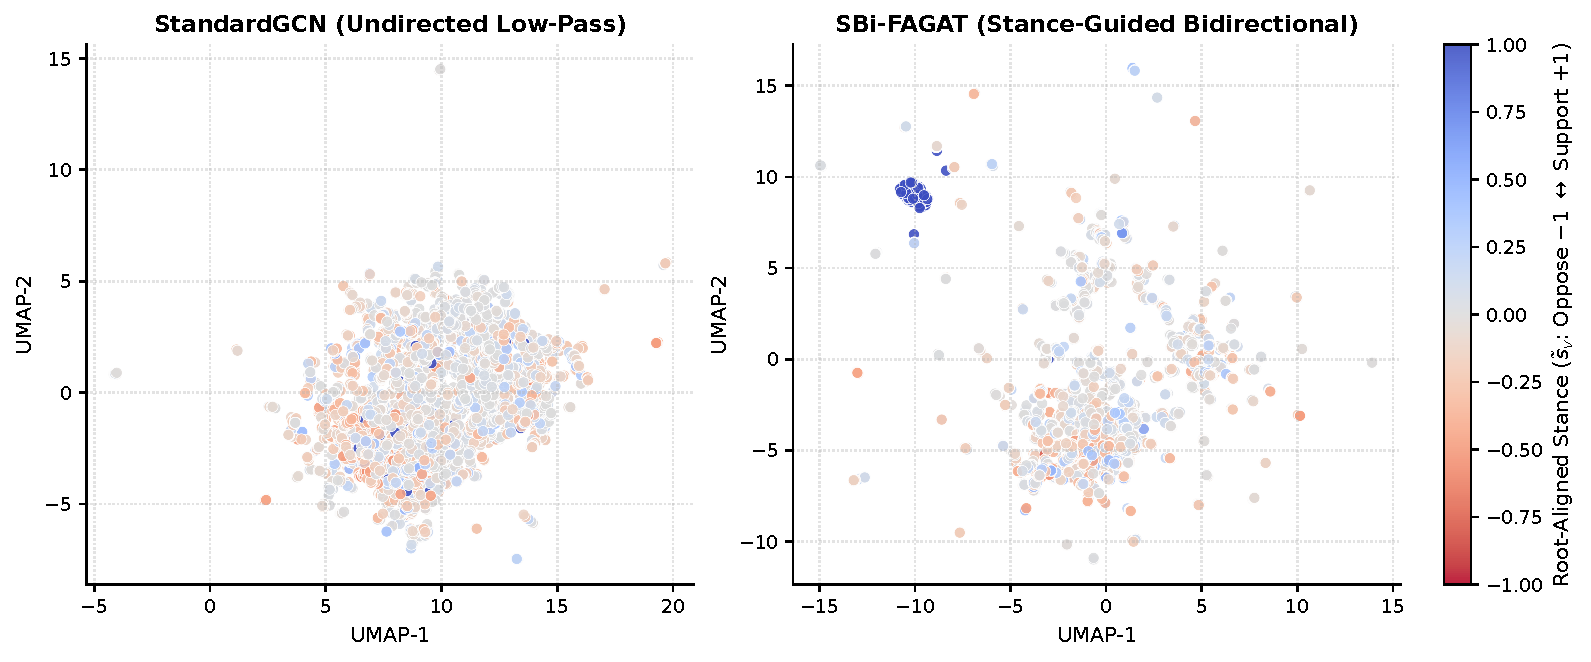
\includegraphics[width=\textwidth]{figures/vn/fig1_umap_polarization.pdf}
\caption{Vietnamese Reddit Test UMAP Node Embeddings: \texttt{StandardGCN} (left) vs.\ \texttt{SBiFAGAT} (right), colored by root-aligned stance polarity.}
\label{fig:umap_vn}
\end{figure*}
}{}

\IfFileExists{figures/pheme/fig1_umap_polarization.pdf}{
\begin{figure*}[t]
\centering
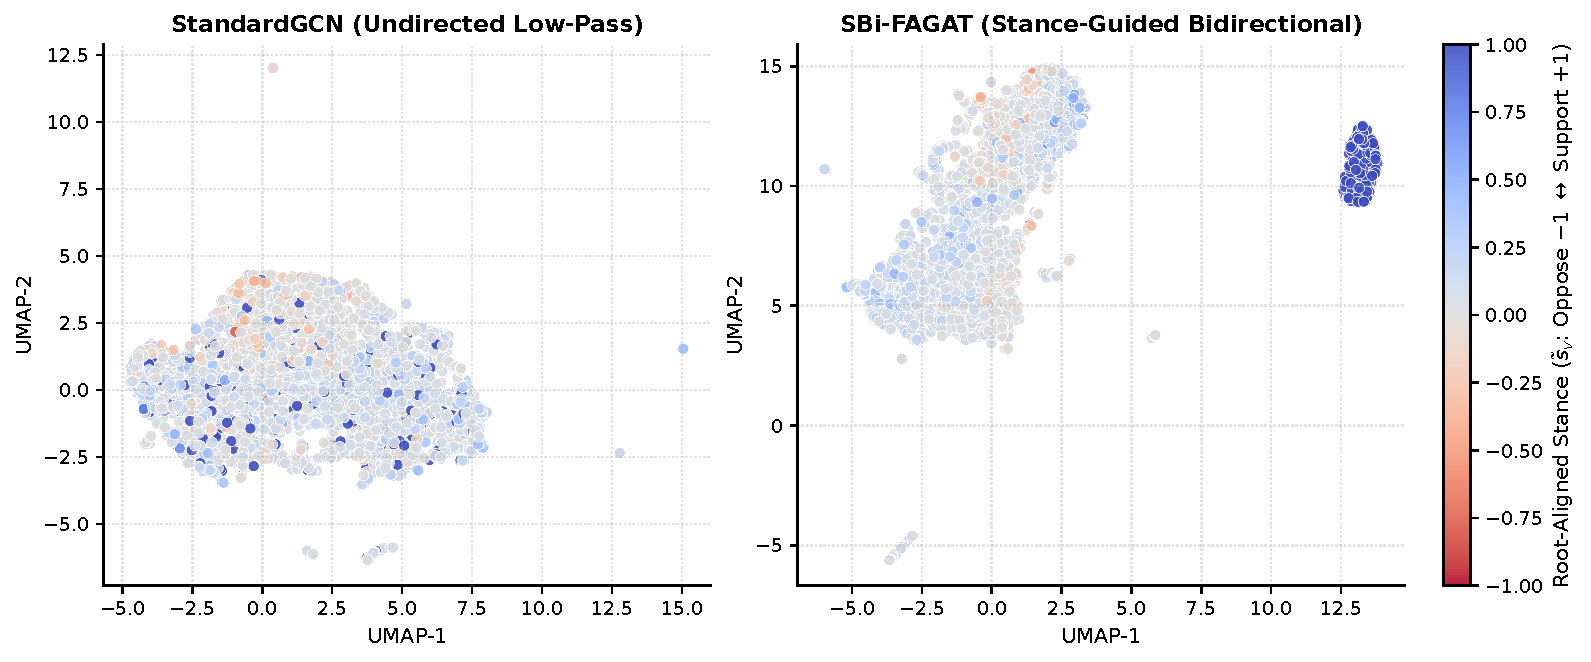
\includegraphics[width=\textwidth]{figures/pheme/fig1_umap_polarization.pdf}
\caption{PHEME Test UMAP Node Embeddings: \texttt{StandardGCN} (left) vs.\ \texttt{SBiFAGAT} (right), colored by root-aligned stance polarity.}
\label{fig:umap_pheme}
\end{figure*}
}{}

\IfFileExists{figures/vn/fig2_early_k_curve.pdf}{
\begin{figure*}[t]
\centering
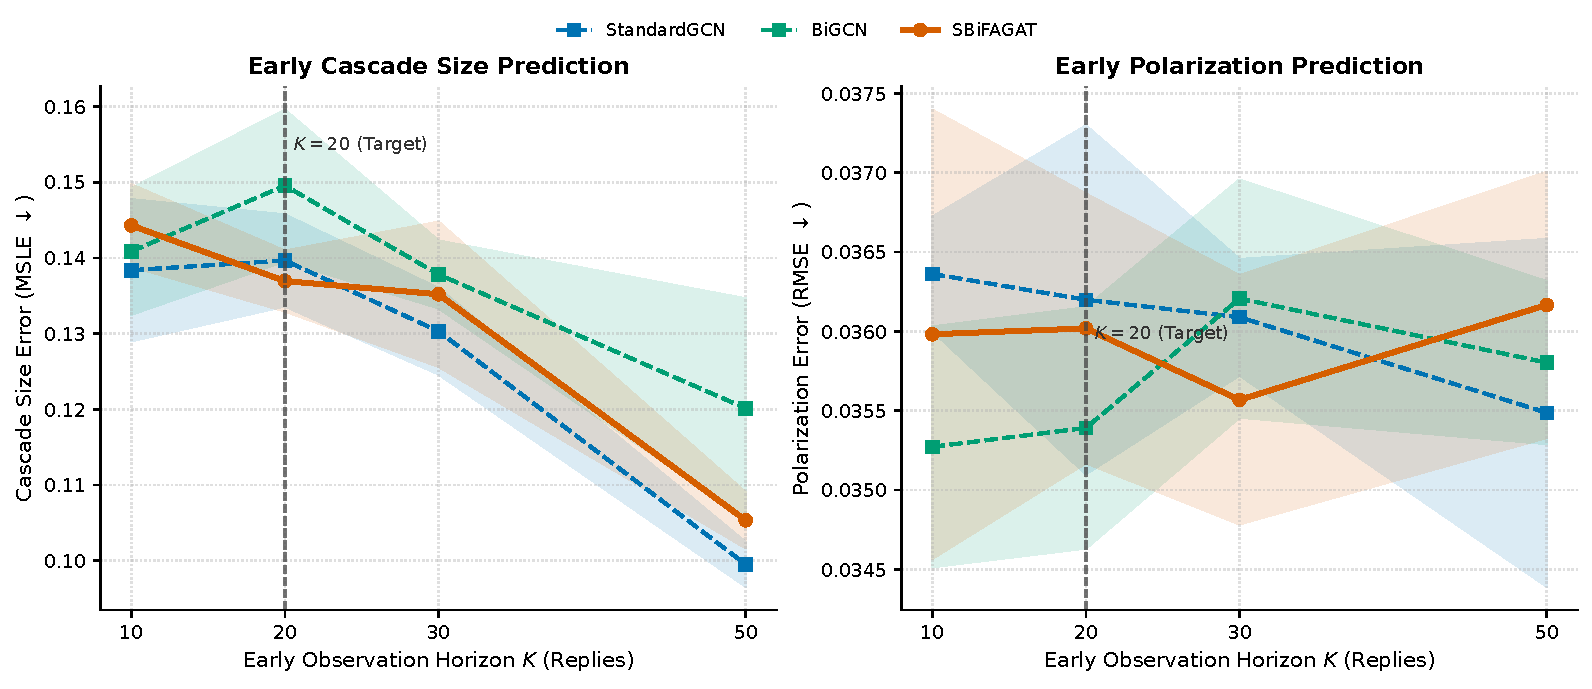
\includegraphics[width=\textwidth]{figures/vn/fig2_early_k_curve.pdf}
\caption{Vietnamese Reddit Early Horizon Sensitivity ($K \in \{10, 20, 30, 50\}$) on the common fixed-future subset ($N_{\text{reply}} \ge 55$, evaluating unobserved future replies past reply index $k > 50$).}
\label{fig:k_curve_vn}
\end{figure*}
}{}

\IfFileExists{figures/pheme/fig2_early_k_curve.pdf}{
\begin{figure*}[t]
\centering
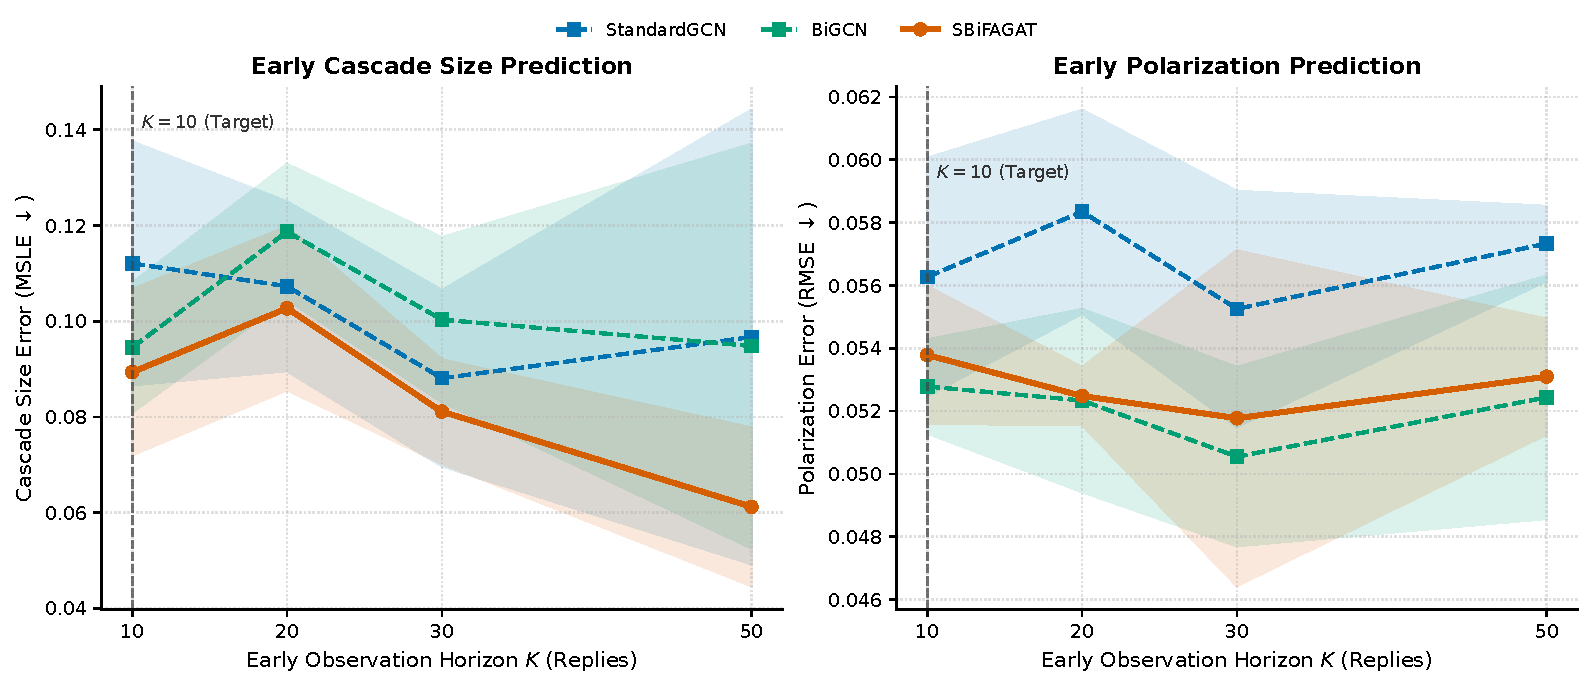
\includegraphics[width=\textwidth]{figures/pheme/fig2_early_k_curve.pdf}
\caption{PHEME Early Horizon Sensitivity ($K \in \{10, 20, 30, 50\}$) on the common fixed-future subset ($N_{\text{reply}} \ge 55$, evaluating unobserved future replies past reply index $k > 50$, $n=10$ Test cascades).}
\label{fig:k_curve_pheme}
\end{figure*}
}{}

\IfFileExists{figures/vn/fig3_cascade_heatmap.pdf}{
\begin{figure*}[t]
\centering
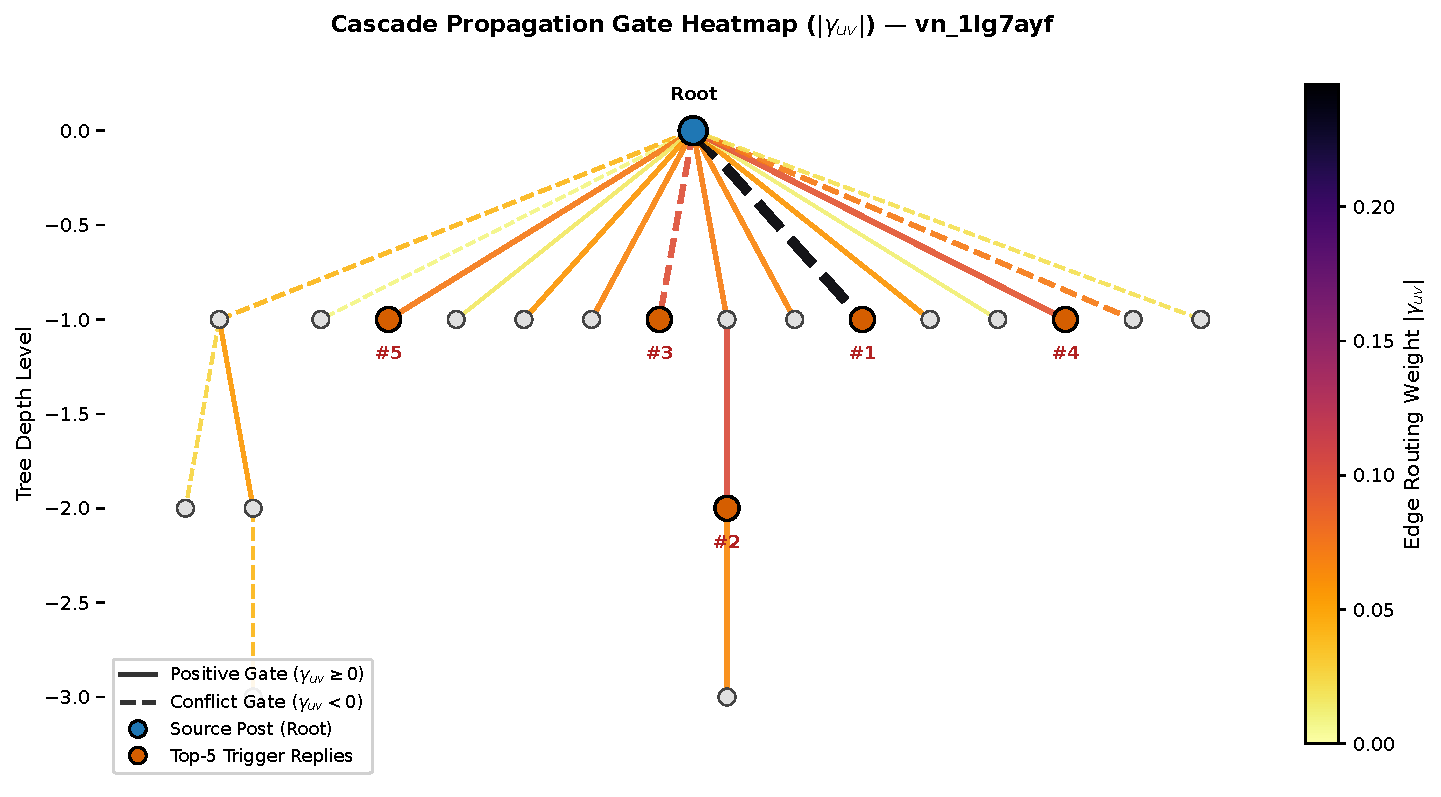
\includegraphics[width=0.92\textwidth]{figures/vn/fig3_cascade_heatmap.pdf}
\caption{Vietnamese Reddit High-Polarization Cascade Gate Heatmap ranking early replies by $|\gamma_{uv}|$.}
\label{fig:heatmap_vn}
\end{figure*}
}{}

\IfFileExists{figures/pheme/fig3_cascade_heatmap.pdf}{
\begin{figure*}[t]
\centering
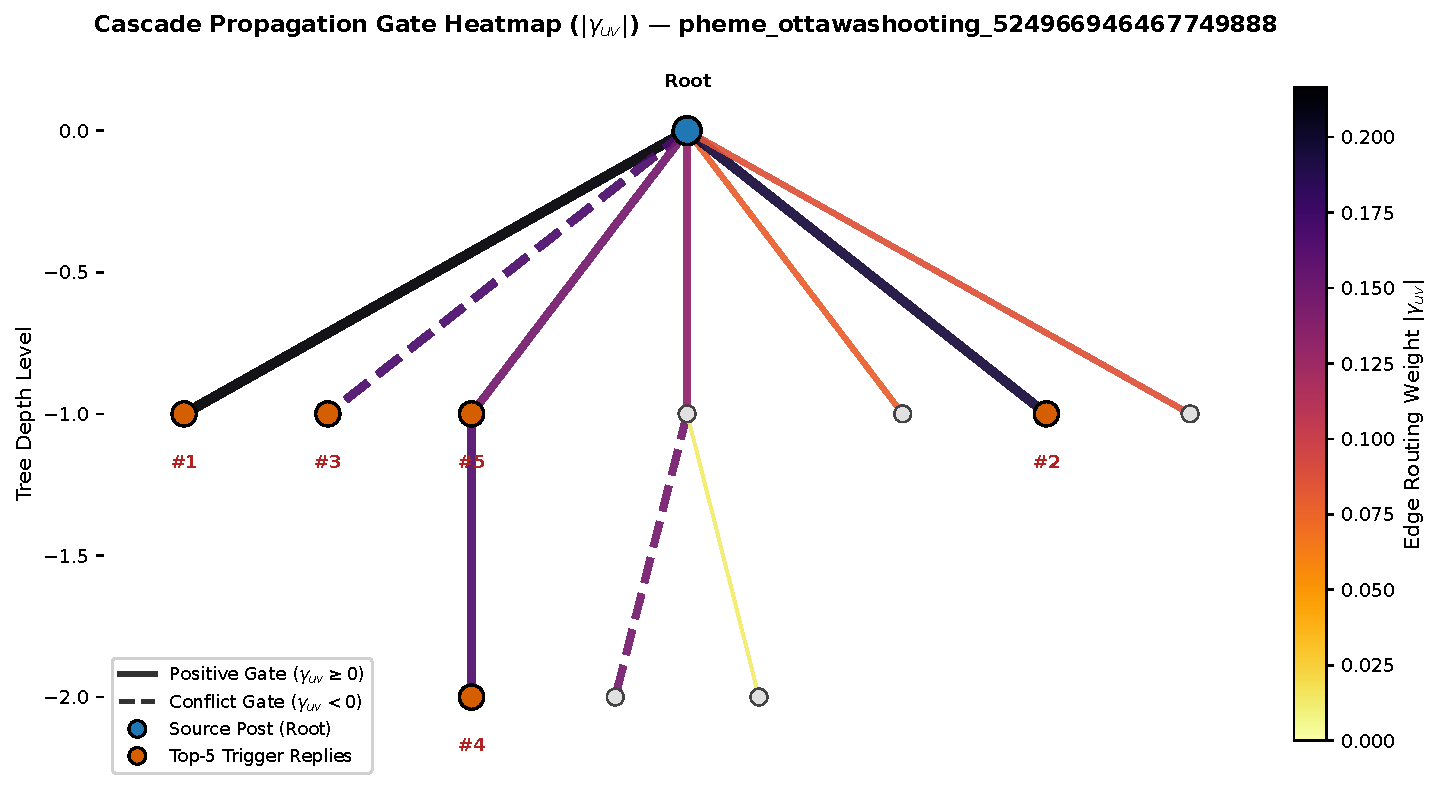
\includegraphics[width=0.92\textwidth]{figures/pheme/fig3_cascade_heatmap.pdf}
\caption{PHEME High-Polarization Cascade Gate Heatmap ranking early replies by $|\gamma_{uv}|$.}
\label{fig:heatmap_pheme}
\end{figure*}
}{}

\IfFileExists{figures/vn/fig4_counterfactual_interventions.pdf}{
\begin{figure*}[t]
\centering
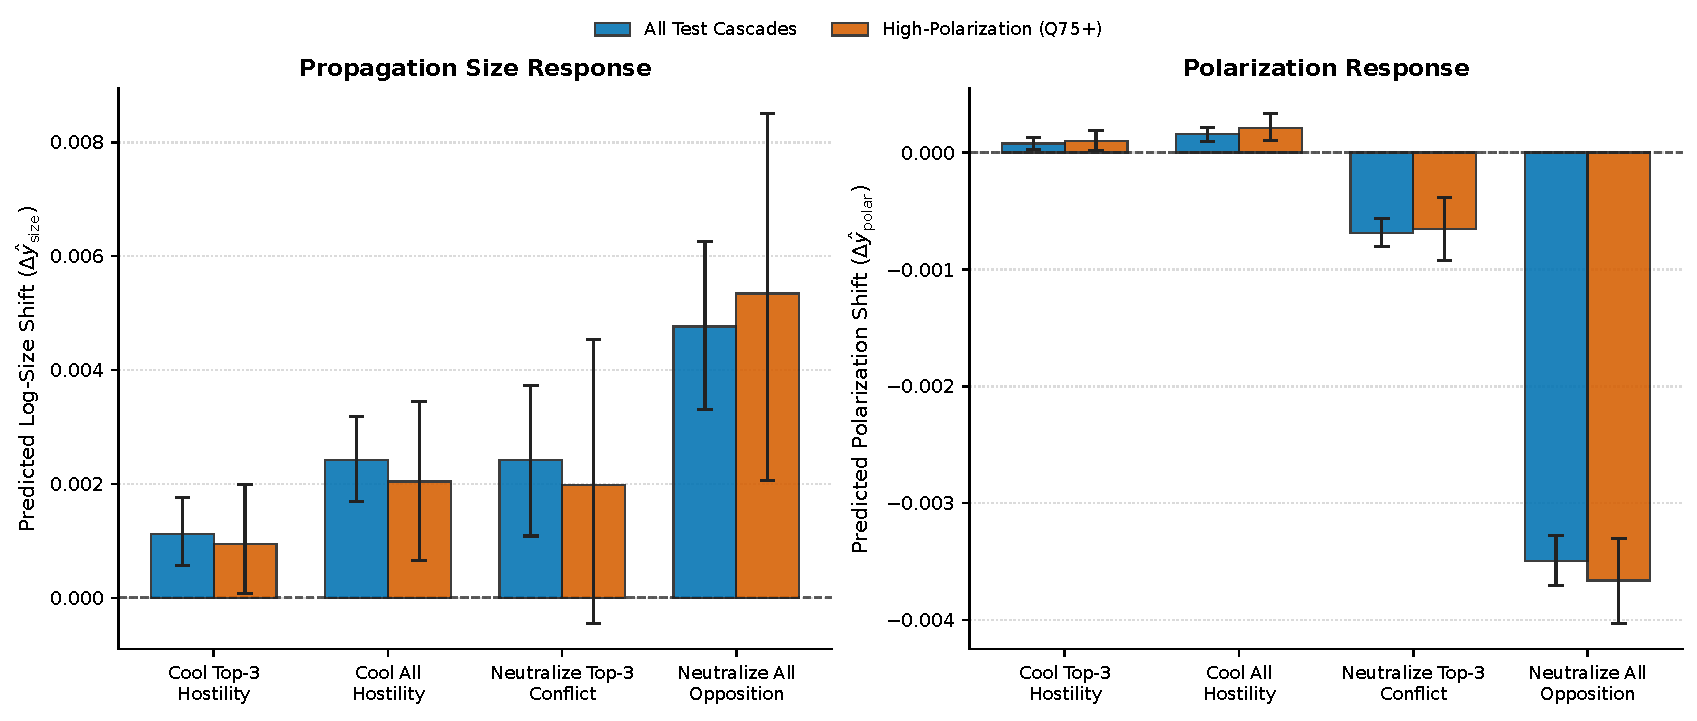
\includegraphics[width=0.92\textwidth]{figures/vn/fig4_counterfactual_interventions.pdf}
\caption{Vietnamese Reddit Observational Edge-Feature Sensitivity Probe across All Test and Top-Quartile (75th+ percentile) cohorts with 95\% paired bootstrap CIs.}
\label{fig:cf_vn}
\end{figure*}
}{}

\IfFileExists{figures/pheme/fig4_counterfactual_interventions.pdf}{
\begin{figure*}[t]
\centering
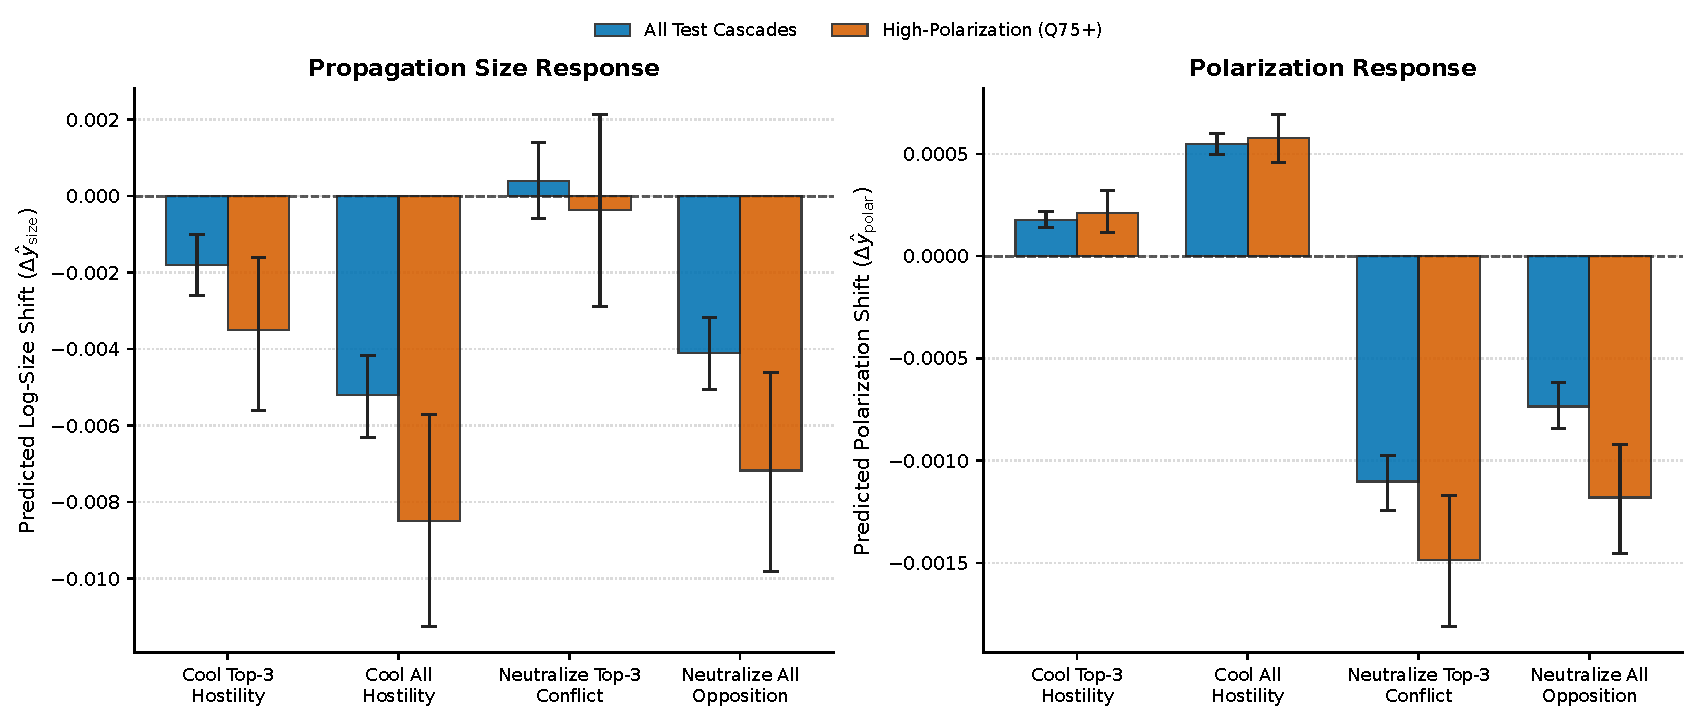
\includegraphics[width=0.92\textwidth]{figures/pheme/fig4_counterfactual_interventions.pdf}
\caption{PHEME Observational Edge-Feature Sensitivity Probe across All Test and Top-Quartile (75th+ percentile) cohorts with 95\% paired bootstrap CIs.}
\label{fig:cf_pheme}
\end{figure*}
}{}

\IfFileExists{tables_mechanisms_vn.tex}{
  {\setlength{\tabcolsep}{1.2pt}
  \begin{table*}[t]
\centering
\caption{Observational Edge-Feature Sensitivity Analysis on VN Test Cascades (Non-Causal Input Perturbation Mean Shift with 95\% Paired Bootstrap CI).}
\label{tab:mechanisms_vn}
\begin{tabular}{lcccc}
\toprule
Edge-Feature Perturbation & All Test $\Delta \hat{y}_{\mathrm{size}}$ & All Test $\Delta \hat{y}_{\mathrm{polar}}$ & Q75+ $\Delta \hat{y}_{\mathrm{size}}$ & Q75+ $\Delta \hat{y}_{\mathrm{polar}}$ \\
\midrule
Cool Top-3 Trigger Hostility & $+0.0011$ $[+0.0006, +0.0018]$ & $+0.0001$ $[+0.0000, +0.0001]$ & $+0.0009$ $[+0.0001, +0.0020]$ & $+0.0001$ $[+0.0000, +0.0002]$ \\
Cool All Early Hostility & $+0.0024$ $[+0.0017, +0.0032]$ & $+0.0002$ $[+0.0001, +0.0002]$ & $+0.0020$ $[+0.0007, +0.0035]$ & $+0.0002$ $[+0.0001, +0.0003]$ \\
Neutralize Top-3 Trigger Conflict & $+0.0024$ $[+0.0011, +0.0037]$ & $-0.0007$ $[-0.0008, -0.0006]$ & $+0.0020$ $[-0.0004, +0.0045]$ & $-0.0007$ $[-0.0009, -0.0004]$ \\
Neutralize All Opposition & $+0.0048$ $[+0.0033, +0.0063]$ & $-0.0035$ $[-0.0037, -0.0033]$ & $+0.0053$ $[+0.0021, +0.0085]$ & $-0.0037$ $[-0.0040, -0.0033]$ \\
\bottomrule
\end{tabular}
\end{table*}
}
}{}

\IfFileExists{tables_mechanisms_pheme.tex}{
  {\setlength{\tabcolsep}{1.2pt}
  \begin{table*}[t]
\centering
\caption{Observational Edge-Feature Sensitivity Analysis on PHEME Test Cascades (Non-Causal Input Perturbation Mean Shift with 95\% Paired Bootstrap CI).}
\label{tab:mechanisms_pheme}
\begin{tabular}{lcccc}
\toprule
Edge-Feature Perturbation & All Test $\Delta \hat{y}_{\mathrm{size}}$ & All Test $\Delta \hat{y}_{\mathrm{polar}}$ & Q75+ $\Delta \hat{y}_{\mathrm{size}}$ & Q75+ $\Delta \hat{y}_{\mathrm{polar}}$ \\
\midrule
Cool Top-3 Trigger Hostility & $-0.0018$ $[-0.0026, -0.0010]$ & $+0.0002$ $[+0.0001, +0.0002]$ & $-0.0035$ $[-0.0056, -0.0016]$ & $+0.0002$ $[+0.0001, +0.0003]$ \\
Cool All Early Hostility & $-0.0052$ $[-0.0063, -0.0042]$ & $+0.0005$ $[+0.0005, +0.0006]$ & $-0.0085$ $[-0.0113, -0.0057]$ & $+0.0006$ $[+0.0005, +0.0007]$ \\
Neutralize Top-3 Trigger Conflict & $+0.0004$ $[-0.0006, +0.0014]$ & $-0.0011$ $[-0.0012, -0.0010]$ & $-0.0004$ $[-0.0029, +0.0021]$ & $-0.0015$ $[-0.0018, -0.0012]$ \\
Neutralize All Opposition & $-0.0041$ $[-0.0051, -0.0032]$ & $-0.0007$ $[-0.0008, -0.0006]$ & $-0.0072$ $[-0.0098, -0.0046]$ & $-0.0012$ $[-0.0015, -0.0009]$ \\
\bottomrule
\end{tabular}
\end{table*}
}
}{}

\end{document}
